\documentclass[12pt]{article}
\usepackage[square,numbers]{natbib}     % package utilisé pour la partie de référence
\bibliographystyle{plainnat}
\usepackage[utf8x]{inputenc}
\usepackage[french]{babel}
\usepackage{caption}
\usepackage{subcaption}
\usepackage{url}
\usepackage{amsmath}
\usepackage{graphicx}
\graphicspath{{images/}}
\usepackage{parskip}
\usepackage{fancyhdr}
\usepackage{vmargin}
\usepackage[T1]{fontenc}

%Configuration pour les codes insérés
\usepackage{listings}

% Ce package est pour définir les couleurs de texte
\usepackage{xcolor}
%\usepackage{color}
\definecolor{codegreen}{rgb}{0,0.6,0}
\lstset{frame=tb,
  language=Java,
  aboveskip=3mm,
  belowskip=3mm,
  showstringspaces=false,
  columns=flexible,
  basicstyle={\small\ttfamily},
  numbers=none,
  numberstyle=\tiny\color{gray},
  keywordstyle=\color{blue},
  commentstyle=\color{codegreen},
  stringstyle=\color{black},
  breaklines=true,
  breakatwhitespace=true,
  tabsize=3
}


% utiliser pour faire annexe https://www.jujens.eu/posts/2013/Oct/20/latex-annexe/
% [titletoc permet d'afficher dans le table of contents]
\usepackage[titletoc]{appendix}

% make a clibable table of content
\usepackage[colorlinks=false]{hyperref}

% enlever les bordures de table des matières
\hypersetup{%
    pdfborder = {0 0 0}
}

%Includes "References" in the table of contents
\usepackage[nottoc]{tocbibind}

\usepackage{float} % utiliser cet package pour insérer les figures, permet de mettre juste après le texte



%change paragraph indent
\setlength{\parindent}{2em}

% Utiliser pour spécifier la liste itemize
\usepackage{enumitem}

\usepackage{array}%%pour tableau

\usepackage{vmargin}
%1 est la marge gauche
%2 est la marge en haut
%3 est la marge droite
%4 est la marge en bas
%5 fixe la hauteur de l’entête
%6 fixe la distance entre l’entête et le texte
%7 fixe la hauteur du pied de page
%8 fixe la distance entre le texte et le pied de page
\setmarginsrb{3 cm}{2.5 cm}{3 cm}{2.5 cm}{2 cm}{1.5 cm}{1 cm}{1.5 cm}

\title{\textbf{Rapport de projet de fin d'études\newline \hfill\\ Automatisation de Test fonctionnel}}    % Title
\author{ZHANG Qilin}		% Author
\date{Septembre 2019}				% Date

\makeatletter
\let\thetitle\@title
\let\theauthor\@author
\let\thedate\@date
\makeatother

\pagestyle{fancy}
\fancyhf{}
\usepackage{lastpage}


\setcounter{tocdepth}{3} % Set the depth of table of contents
\setcounter{page}{3}
\begin{document}

%%%%%%%%%%%%%%%%%%%%%%%%%%%%%%%%%%%%%%%%%%%%%%%%%%%%%%%%%%%%%%%%%%%%%%%%%%%
%Title
\begin{titlepage}
	\centering
    \vspace*{0.5 cm}
    \begin{figure}
        \begin{subfigure}{0.3\textwidth}
        \flushleft
            
\includegraphics[width=\textwidth]{Logo_officiel_Sorbonne_University.png}
        \end{subfigure}
        \hspace{.4\textwidth}
        \begin{subfigure}{0.3\textwidth}
            
\includegraphics[width=\textwidth]{SAP_R_grad.jpg}
        \end{subfigure}
    \end{figure}
    \textsc{\LARGE Sorbonne Université}\\[2.0 cm]	% University Name
	\textsc{\Large Master 2 Science et Technologie du Logiciel\\2018 - 2019}\\[0.5 cm]		% Course Code
	%\textsc{\large Développement d'Application Réticulaire }\\[0.5 cm]	% Course Name
	\rule{\linewidth}{0.8 mm} \\[0.6 cm]
	{ \huge \bfseries \thetitle}\\[0.6 cm]
	\rule{\linewidth}{0.8 mm} \\[2.6 cm]

	\begin{minipage}{0.4\textwidth}
		\begin{flushleft} \large
			\emph{Etudiants:}\\
			\theauthor
			\end{flushleft}
			\end{minipage}~
			\begin{minipage}{0.4\textwidth}
			\begin{flushright} \large
			\emph{Tuteurs:} \\
			CHRISTIANSEN Camilla, COUDRAY Sébastien % Your Student Number
		\end{flushright}
	\end{minipage}\\[1.6 cm]
	 
	{\large \thedate}\\[2 cm]
 
	\vfill
	
\end{titlepage}

%%%%%%%%%%%%%%%%%%%%%%%%%%%%%%%%%%%%%%%%%%%%%%%%%%%%%%%%%%%%%%%%%%%%%%%%%%%%%%%%%%%%%%%%%
\null
\newpage
%%%%%%%%%%%%%%%%%%%%%%%%%%%%%%%%%%%%%%%%%%%%%%%%%%%%%%%%%%%%%%%%%
\pagenumbering{roman} % Start roman numbering

%% set thing show in right and left head and foot of page
\rhead{\rightmark}
\lhead{Sorbonne Université Master 2 STL\newline \theauthor}
\cfoot{\thepage}

%% set head and foot rule
\renewcommand{\headrulewidth}{2pt}
\renewcommand{\footrulewidth}{1pt}

%tables des matières
\tableofcontents
\pagebreak

%Listes des figures et talbeaux
\listoffigures
\listoftables

\pagebreak

%%%%%%%%%%%%%%%%%%%%%%%%%%%%%%%%%%%%%%%%%%%%%%%%%%%%%%%%%%%%%%%%%%%%%%%%%%%%%%%%%%%%%%%
\pagenumbering{arabic} % Start roman numbering

\cfoot{Page \thepage \ sur\ \pageref{LastPage}}
\newpage

\section{Remerciements}
Je tiens tout d'abord à remercier toutes les personnes qui m'ont aidé au succès de mon alternance de cette année et de la rédaction de ce mémoire.

\par Je voudrais dans un premier temps remercier à l'ensemble de l'équipe Finance France de SAP France, pour son accueil et sa bienveillance tout au long de l'année. Je tiens à remercier particulièrement des personnes suivantes : 
\begin{itemize}
    \item Mes tuteurs, Monsieur Sébastien Coudray, Developer Senior, et Madame Camilla Christiansen, Senior Quality Specialist, avec qui que je travaille tout au long de l'année, pour leurs esprits professionnels, leurs patiences pour m'expliquer et m'aider pour mon travail.
    \item Monsieur David Dufour, Development Senior Manager IMS, pour son implication dans mon recrutement au sein de SAP France.
    \item Monsieur Thibault Lefaix, Development Manager, pour son explication qui m'a beaucoup aidé à comprendre l'architecture Financial Consolidation et à finir cette mémoire.
    \item Monsieur Thierry Gosselin, Quality Expert, Scrum Master, pour sa façon de gérer l'équipe et le projet Financial Consolidation.
\end{itemize}

\par Mes remerciements ne sont pas envoyées que les personnes indiquées dans la liste précédentes, y contient aussi tous les collègues d'équipe, durant cette année de travail, ils m'ont aidé à bien "On-Boarding" à SAP France, m'ont aidé à déboguer mes programmes, m'ont pris le temps pour discuter mon sujet d'alternance. 

\par Je remercie également toute l'équipe pédagogique de Sorbonne Université et de CFA-INSTA, particulièrement monsieur Binh-Minh Bui-Xuan et monsieur Emmanuel Chailloux pour leurs conseils
tout au long de l’année, madame Emilie Auger pour son travail administrative de la promotion. Je remercie aussi la promotion M2 STL 2018 auprès de laquelle j’ai passé une année formidable.

\par Enfin, je pense à mes proches, mes meilleurs amis, qui m'ont encouragé et soutenu pour ma vie et mes études en France tout au long de ces années.

%%%%%%%%%%%%%%%%%%%%%%%%%%%%%%%%%%%%%%%%%%%%%%%%%%%%%%%%%%%%%%%%%%%%%%%%%%%%%%%%%%%%%%%%%
\newpage

\section{Introduction}
\subsection{Cadre}
Ce rapport est écrit dans le cadre de ma formation en Master 2 Informatique, spécialité de Science et Technologie du Logiciel à Sorbonne Université, dans ce cadre, j'effectue une année d'alternance entre un parcours théorique auprès des intervenants et professeurs à Sorbonne Université et à CFA INSTA (Institut National Supérieur des Technologies Avancées), et une expérience professionnelle chez SAP France en tant que développeur de test automatisé.


\subsection{Organisation du rapport}
Ce rapport décrit l'essentiel de contenu de mon alternance, il est divisé globalement en trois parties : 
    \begin{enumerate}
        \item La première partie fait une présentation d'organisation où j'effectue mon alternance, il parle de SAP SE, de SAP France et l'équipe dans lequel je travail.
        \item La deuxième partie décrit le contexte et la problématique du projet : Automatisation des tests d'impressions de l'application \textit{SAP Financial Consolidation} Client Web HTML5. 
        \item La troisième partie parle des travaux que j'ai réalisé, il décrit la solution qui a été développé pour résoudre le problème de la deuxième partie.
    \end{enumerate} 
\newpage


\section{Présentation d'entreprise}

\subsection{Vue globale}
    \par SAP SE (\textit{\textbf{S}ysteme, \textbf{A}nwendungen und \textbf{P}rodukte in der Datenverarbeitung}, "\textit{\textbf{S}ystems, \textbf{A}pplications \& \textbf{P}roducts in Data Processing}") est une entreprise qui conçoit et vend des logiciels, notamment des systèmes de gestion et de maintenance, principalement à destination des entreprises et des institutions dans le monde entier. Elle est fondée par 5 anciens employés d’IBM - Dietmar Hopp, Hans-Werner Hector,Hasso Plattner, Klaus E. Tschira, et Claus Wellenreuther en 1972. SAP est une entreprise internationale et sont siège se localise à Waldorf, Allemagne.
    
    \par \cite{SAP_Corporate_Fact_Sheet} SAP est le premier éditeur de logiciels en Europe et le quatrième dans le monde. SAP a 98332 employés au tour du monde dans plus de 147 pays jusqu'à 30 Juin 2019. La stratégie de SAP est "The best-run business", le quel SAP veut aider le monde et améliorer la vie de tout le monde. SAP fournit les services pour plus de 437000 clients dans plus de 180 pays, 92\% des clients sont dans la liste de Forbes Global 2000 companies. Pour l'année 2018, SAP a une revenue globale de 24,47 billons euros (non-IFRS) au tour du monde.
    \begin{figure}[H]
        \flushleft
        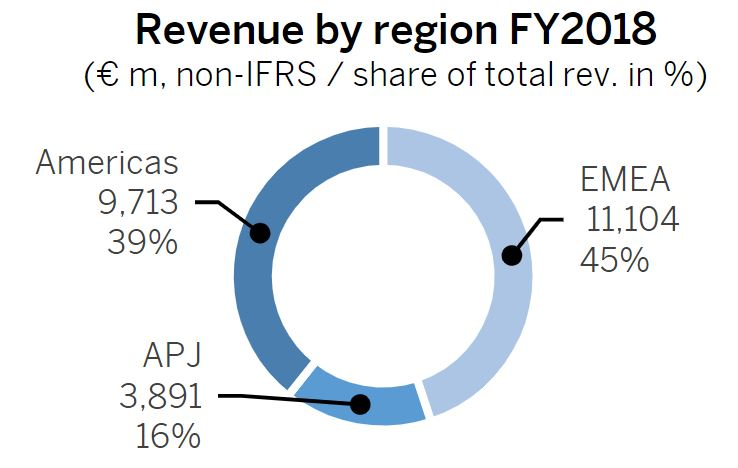
\includegraphics[width=.5\textwidth]{sap_revenu_by_region.JPG}
        \caption{Revenue par région FY2018}
        \label{fig:revenue_by_region2018_label}
    \end{figure}
    
\newpage    
%\subsection{Histoire}
%    (Source : \citet{SAP-History})
%    \subsubsection{Années 1972 - 1980: Les jeunes années}
%    En 1972, 5 anciens employés d'IBM - Dietmar Hopp, Hans-Werner Hector, Hasso Plattner, Klaus E. Tschira, et Claus Wellenreuther - fondaient Systems Applications and Products in Data Processing (Systèmes, Applications et Progiciels), à Mannheim, en Allemagne. S'appuyant sur le rêve de l'informatique «temps réel»: un logiciel qui traite les données lorsque les clients en ont besoin plutôt que de passer la nuit à la volée. SAP a délivré la release SAP R/1 en 1973.
%
%    \subsubsection{Années 1981 - 1990 : Le SAP R/2}
%    Le temps réel touche davantage l’activité: les processus d’application logicielle mainframe packagés SAP R/2 intègrent l’ensemble des fonctions commerciales d’une entreprise.
%
%    \subsubsection{Années 1991 - 2000 : Le SAP R/3}
%    Temps réel sur le bureau: une version client-serveur du logiciel d'application standard permet aux entreprises de fonctionner plus efficacement dans le monde entier.
%    \subsubsection{Années 2001 - 2010 : Des données en temps réel}
%    Déplacements vers le Web en temps réel et au-delà: l'informatique en nuage, mobile et en mémoire ouvrent de nouveaux horizons pour l'accès aux données en temps réel, où que vous soyez et quand vous en avez besoin.
%    
%    \subsubsection{Années 2011 - Présent : SAP HANA, Cloud}
%    La croissance continue de l'entreprise est tirée par la plate-forme en mémoire SAP HANA qui permet aux analyses de données ultra-rapides de devenir une réalité. Des acquisitions stratégiques associées à une innovation continue font de SAP un leader des réseaux d’informatique en nuage et du commerce électronique. Avec le lancement de SAP S / 4HANA et de SAP C / 4HANA, SAP dévoile la nouvelle génération de logiciels d'entreprise destinés à aider les clients à devenir des entreprises intelligentes.
%
\subsection{Commerce de SAP} 
\subsubsection{Activités et marchés}
\cite{SAP-entreprise_wikipedia}SAP opère dans trois zones géographiques : Europe/Moyen-Orient/Afrique (\textbf{EMEA}), \textbf{Amériques} (le siège de SAP America, qui regroupe Amérique du Nord et Amérique latine, se trouve à Newtown Square, en Pennsylvanie), et Asie/Pacifique/Japon (\textbf{APJ}, qui regroupe Japon, Australie, Inde et plusieurs autres pays d’Asie). SAP dispose également d’un réseau de 115 filiales, et de cabinets de Recherche \& Développement.

SAP se concentre sur six secteurs : procédés industriels de fabrication, d’assemblage, de distribution et de services aux consommateurs, services financiers et publics. La société propose plus de 25 produits aux grandes entreprises et plus de 550 pour les petites et moyennes entreprises.

\par Comme la portfolio de produit SAP \textbf{\textit{\ref{fig:portfolioSAP_label}}} indique ci-dessous, les produits de SAP divise en 9 parties : 
\begin{itemize}
	\item ERP et cœur numérique
	\item Gestion de la relation client et expérience client
	\item Chaîne logistique digitale
	\item RH et implication du personnel
	\item Outils d'analyse
	\item Technologies intelligentes
\end{itemize} 

\begin{figure}[H]
	\centering
	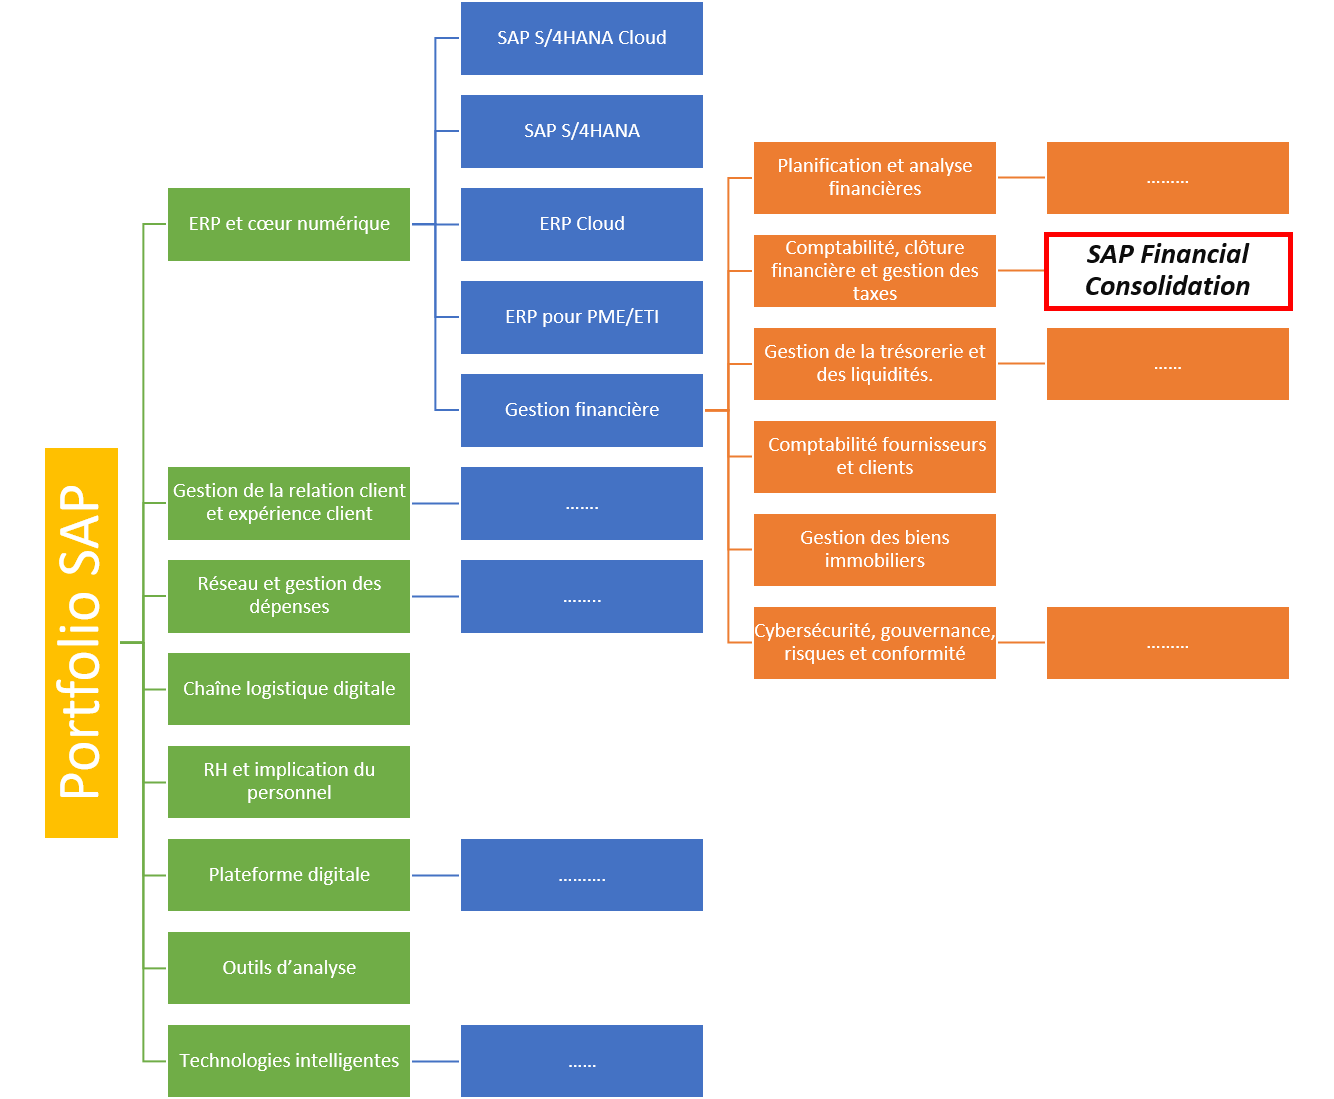
\includegraphics[width=\textwidth]{images/SAP_portfolio.png}
	\caption{Portfolio de SAP}
	\label{fig:portfolioSAP_label}
\end{figure}

Chaque catégorie a plusieurs produits, le produit que je travaille au-dessus s'appelle \textit{SAP Financial Consolidation(FC)}, il est dans la catégorie de Gestion Financière, c'est un produit conçu pour les comptabilités, clôture financières et gestion es taxes. Il y aura une explication de ce produit plus précisé dans la partie \ref{subsec: SAP Fiancial Consolidation}


Les différents départements opérationnels de SAP sont divisés en trois catégories : Recherche \& Développement, activités de terrain et assistance aux consommateurs. SAP Labs conçoit et développe les produits, tandis que des bureaux installés dans chaque pays partenaire se chargent des opérations de terrain comme la vente, le marketing et le conseil. La stratégie et la gestion globale sont décidées et menées au siège de SAP AG, en Allemagne, tout comme le travail d’ingénierie lié à la fabrication des produits.

\subsection{SAP Aujourd'hui et Demain : SAP vers Cloud}
Depuis 2012, SAP a acquis plusieurs sociétés qui vendent des produits dans le cloud pour être compétent dans le marché Cloud. Par exemple : En 2014, SAP a acheté Concur Technologies, un fournisseur de logiciels de gestion des déplacements et des dépenses en nuage

\par SAP a aussi coopéré avec les autres entreprises comme IBM, Microsoft, Google pour mieux fournir les services cloud aux clients. SAP a également investi IOT(Internet of Things) et lancé sa propre cloud solution : SAP HANA Solution. En 2015, SAP a lancé SAP S/4 HANA, une nouvelle génération de SAP Business Suite, ce produit est écrit nativement pour le SAP HANA plate forme .

\subsection{SAP France}
    Après l'acquisition de \textit{BuisinessObjects} en Octobre 2007, SAP SE a fondé sa filiale en France - SAP France. 
    \par Aujourd'hui, SAP France présente plus de 1500 de salarié en temps plein. Le siège local de SAP France est à \textbf{Tour SAP} 35 rue d'Alsace, 92300 Levallois-Perret, où j'effectue mon alternance. SAF France présente aussi un centre de formation et un SAP Labs in Paris qui sont aussi se situent à Tour SAP; 2 bureaux de vente à Lyon et à Toulouse; 2 autres SAP Labs France à Caen et Sophia Antipolis.
    
%    \subsubsection{SAP Labs et SAP Labs Paris}
%    
%     Les SAP Labs sont les principales entités de R\&D de SAP, développant et améliorant constamment les solutions clés de SAP. Ces sites de recherche et développement sont situés de manière stratégique dans des clusters de haute technologie à travers le monde et reflètent la culture de diversité et d’innovation de SAP. Chaque laboratoire met un accent particulier sur les applications spécifiques, la technologie ou le marché. Avec 20 laboratoires dans 17 pays, le \textit{SAP Labs Network} (\textit{SLN}) est un moteur de leadership éclairé au niveau mondial et au sein d'écosystèmes locaux, permettant à SAP d'innover, de se développer et de réussir.
%        \begin{figure}[H]
%            \centering
%            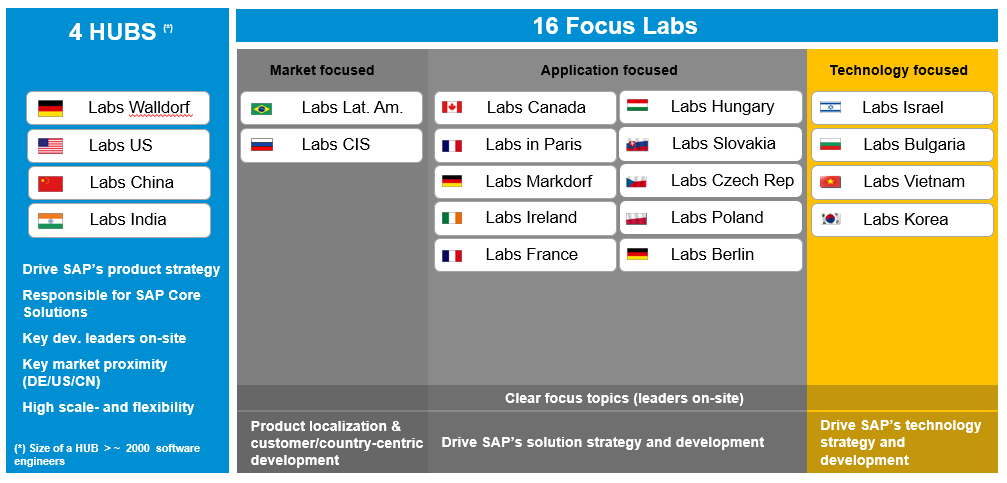
\includegraphics[width=\textwidth]{sap_labs_focus.png}
%            \caption{Focus de SAP Labs}
%            \label{fig:SAP_Labs_Focus_label}
%        \end{figure}
%        
%    \par Fondé en 2009, SAP Labs Paris est une partie de \textit{SLN}, SAP Labs Paris se concentre sur l'application des technologies de SAP, tels que la conversation, l'intelligence artificielle, Machine Learning automatique et l'automatisation intelligence des processus robotiques.
    
    \subsubsection{Equipe Finance}
        L'équipe dans laquelle j'effectue mon alternance se situe à la Tour SAP au 35 rue d'Alsace, 92300 Levallois-Perret, répartie principalement sur le 7ème étage de la tour mais aussi au 9ème étage.
        
        \par L'équipe nommée formellement P\&I S/4HANA LoB Finance France (équipe "Line of Business Finance France" de l’équipe "Product and Innovation S/4HANA"), et communément appelée équipe Finance, fait partie du département P\&I Analytics DW IMS EPM de SAP Labs.  Les SAP Labs sont les principales entités de R\&D de SAP, développant et améliorant constamment les solutions clés de SAP. SAP Labs Paris est fondé en 2009, il se concentre sur l'application des technologies de SAP, tels que la conversation, l'intelligence artificielle, Machine Learning automatique et l'automatisation intelligence des processus robotiques.
        
        \paragraph{Organisation du groupe} L'équipe composée de 43 personnes, David DUFOUR est le manager. Dans cette équipe, une sous-équipe nommée FC (Financial Consolidation) développe le produit éponyme. Les produits qui sont maintenus et développés par cette équipe sont des logiciels d’aide à consolidation financière. David DUROUR est au management de cette équipe, dont je fais partie. 
        %Les missions principales de l’équipe FC sont les maintenance et développement des applications suivantes :
        
        %\begin{itemize}
        %    \item Financial Consolidation (FC)
        %    \item Intercompany
        %    \item Financial Information Management (FIM)
        %    \item Business Planning \& Consolidation (BPC)
        %\end{itemize}
        
        \begin{figure}[H]
            \centering
            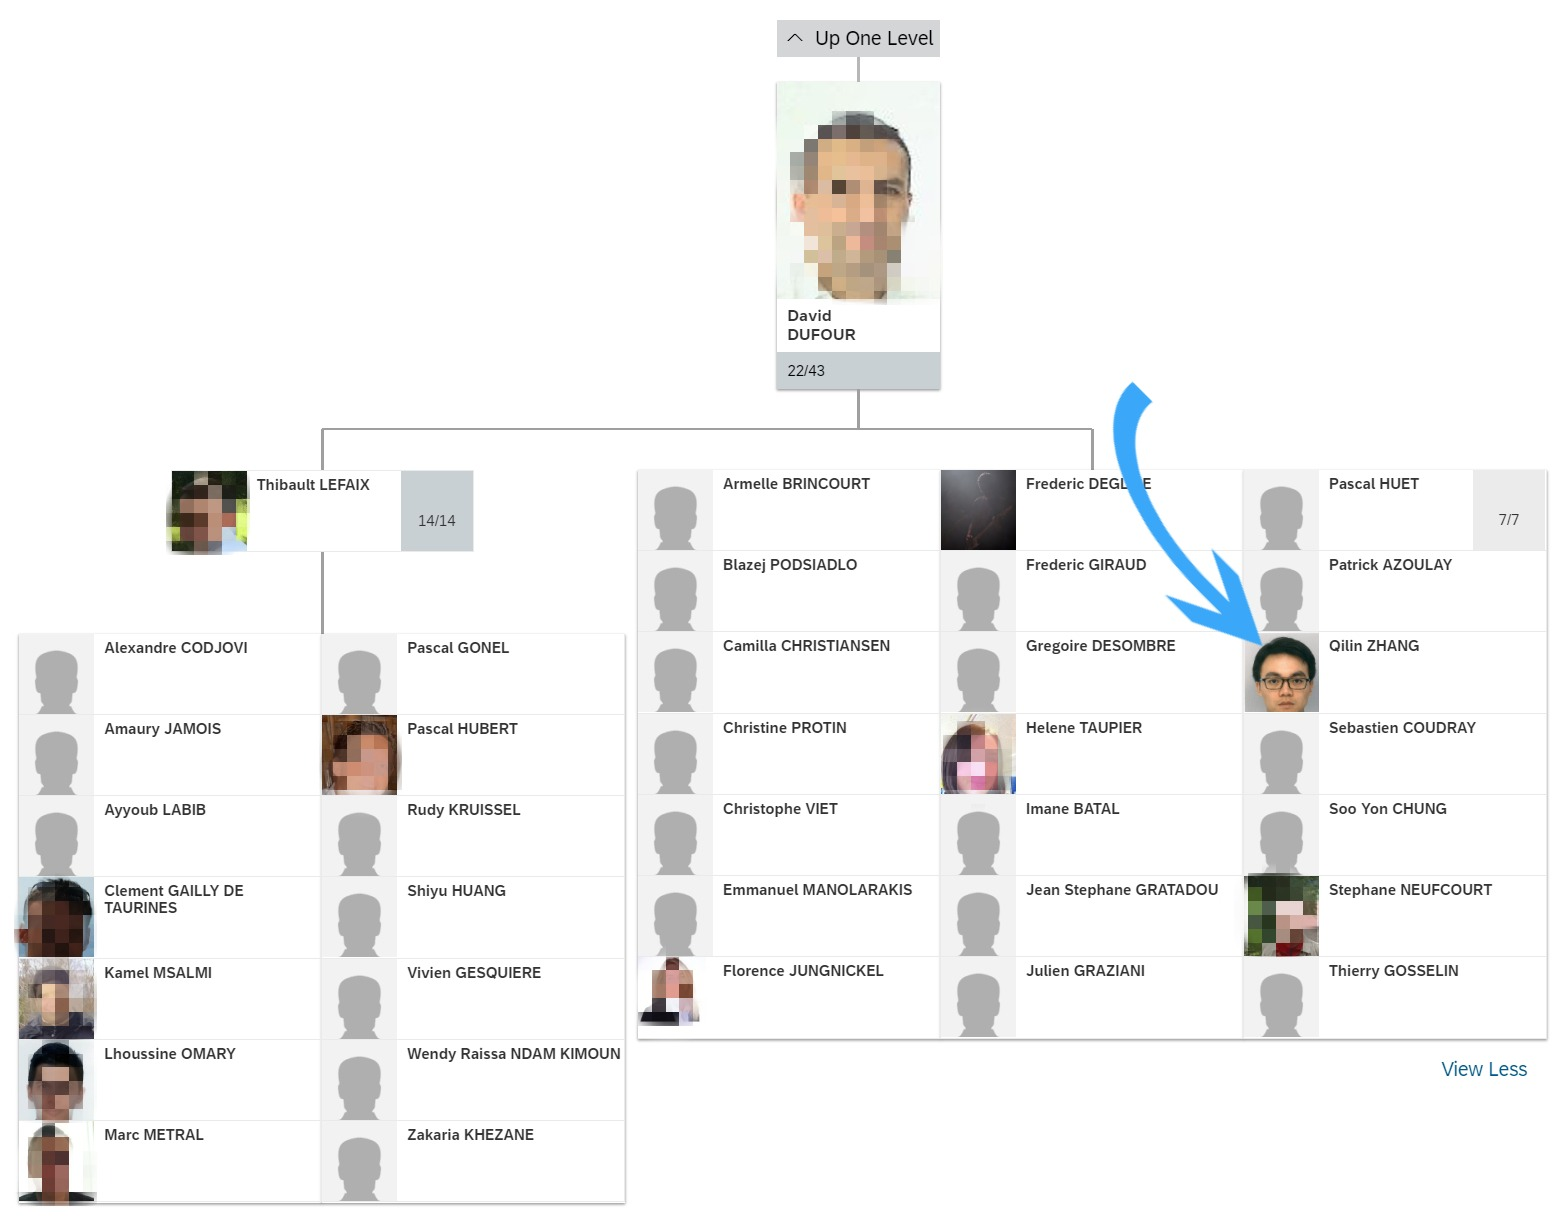
\includegraphics[width=.9\textwidth]{organisation_groupe.jpg}
            \caption{Organisation du groupe}
            \label{fig:group_organization_label}
        \end{figure}
        
        \paragraph{Mon rôle et ma mission}
        Mon rôle durant mon alternance est développeur de test automatisé, Camilla CHRISTIANSEN et un autre Senior Quality Specialist Amaury JAMOIS, qui sont très compétents sur le produit Financial Consolidation rédigent les scénarios de test, je le mets en place et intègre sur notre projet Test-Automatisé. Mon tuteur technique COUDRAY Sébastien va m'expliquer et m'aider à déboguer si je rencontre des difficultés techniques.
%%%%%%%%%%%%%%%%%%%%%%%%%%%%%%%%%%%%%%%%%%%%%%%%%%%%%%%%%%%%%%     
\newpage
\section{Analyse et Compréhension de la problématique}

\subsection{SAP Financial Consolidation}
\label{subsec: SAP Fiancial Consolidation}
\par SAP Financial Consolidation est une application de consolidation légale et de reporting de gestion développé depuis 1999. Il permet aux grandes entreprises de répondre à des exigences de consolidation complexes, de rationaliser la conformité réglementaire, d'unifier le reporting légal et de gestion et d'accélérer le processus de clôture financière global.\cite{About-FC}


\par Avec toutes les évolutions des nouvelles technologies, aujourd'hui SAP Financial Consolidation contient plusieurs versions de clients selon les besoins d'utilisateurs : 
    \begin{description}
        \item [Client Windows Desktop :] Client installer sur Windows
        \item [Client Legacy Web :] Client version Web avant l'utilisation de HTML5
        \item [Client HTML5 Web :] Client version Web avec l'utilisation de HTML5, nouvelle UX.
    \end{description}
    \subsubsection{Architecture}
    
    \paragraph{Architecture globale}
    Le produit SAP Financial Consolidation est conçu et développé comme une \textit{n-tiers application} :
    \begin{itemize}[label=\textbullet]
        \item \textbf{Couche de présentation :} 
            \begin{itemize}
                \item Une ASP .NET web présentation permet de soutenir les HTTP clients légers : Web Client pour entrée de donnée et contrôle de package; Web Admin permet d'avoir une administration au niveau de Web; Excel Web Schedule et Excel Web Links qui est présenté comme un plugin FC dans Excel.
                \item Une nouvelle couche Web de HTML5/SAPUI5 qui est introduise à partie de FC 10.1.
                \item Une couche de Web Service permet d'intégrer avec autres applications : Legacy .NET SOAP Web Service sont utilisés par plusieurs clients de FC et de EPM produits; New .NET REST Web Service pour le nouvel HTML5 Web Client.
            \end{itemize}
        \item \textbf{Couche de traitement :} Le cœur est un \textbf{DCOM} (\textit{Distributed Component Object Model}) \textbf{server} développé en C++ qui permet de communiquer avec la partie Financial Consolidation Server.
        \item \textbf{Couche d'accès aux données :} Une couche d'accès aux bases de données permet d'accéder la base de donnée (SQL Server, Oracle ou SAP Hana).
    \end{itemize}
    
    \begin{figure}[H]
        \centering
        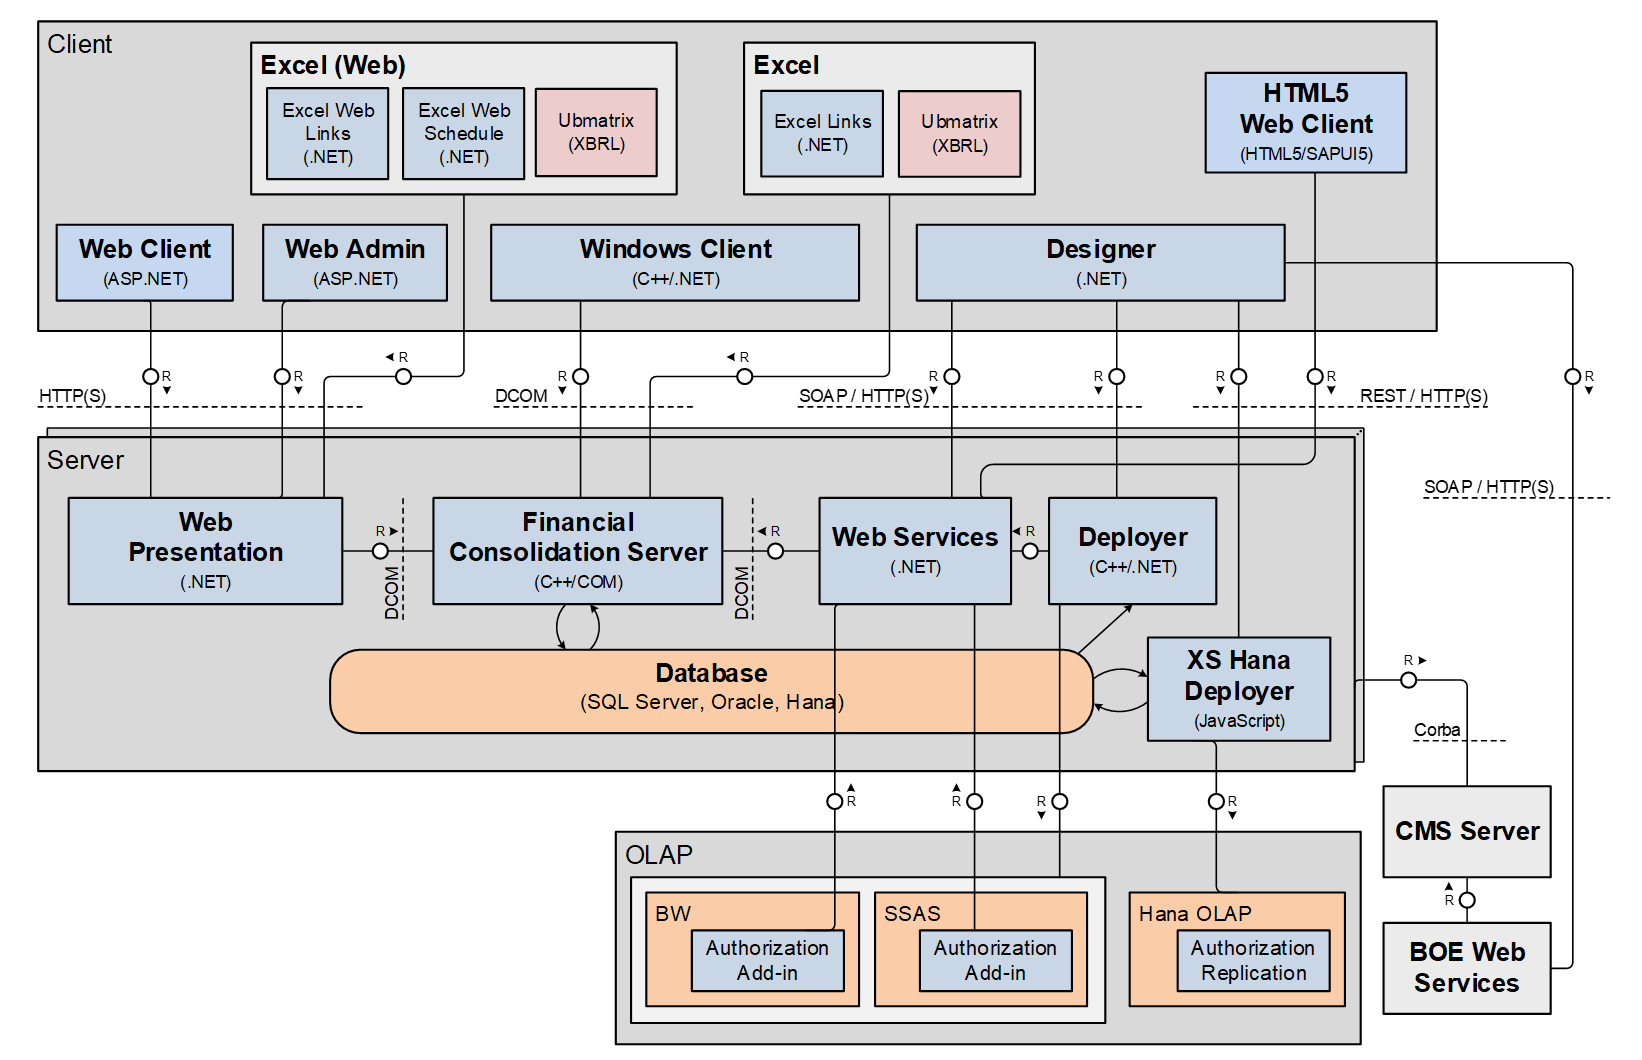
\includegraphics[width=\textwidth]{FC_Globale_Architecture.png}
        \caption{Financial Consolidation architecture globale}
        \label{fig:FC_architecture_label}
    \end{figure}
    
    \paragraph{Architecture du Client HTML5 Web}
    Avec l'évolution des nouvelles technologies et des besoins de nos clients, en plus, il existe beaucoup d’inconvénients pour le client Windows par exemple les traitements sont à locale qui demande beaucoup d'espace sur la machine, en plus, il faut une personne  s'occupe d'installation et de la mise à jour afin d'être cohérent entre deux machines. Avec les raisons ci-dessus, l'équipe a décidé de développer un nouveau client HTML5 Web qui a livré aux clients à partir de la version FC 10.1 pour remplacer l'ancien client Web développé avec ASP .NET. La première version de Client HTML5 Web a été sortie en 2015, l'équipe continue de développer les nouvelles fonctionnalités et de faire les maintenances pour ce client.
    
    \begin{figure}[H]
        \centering
        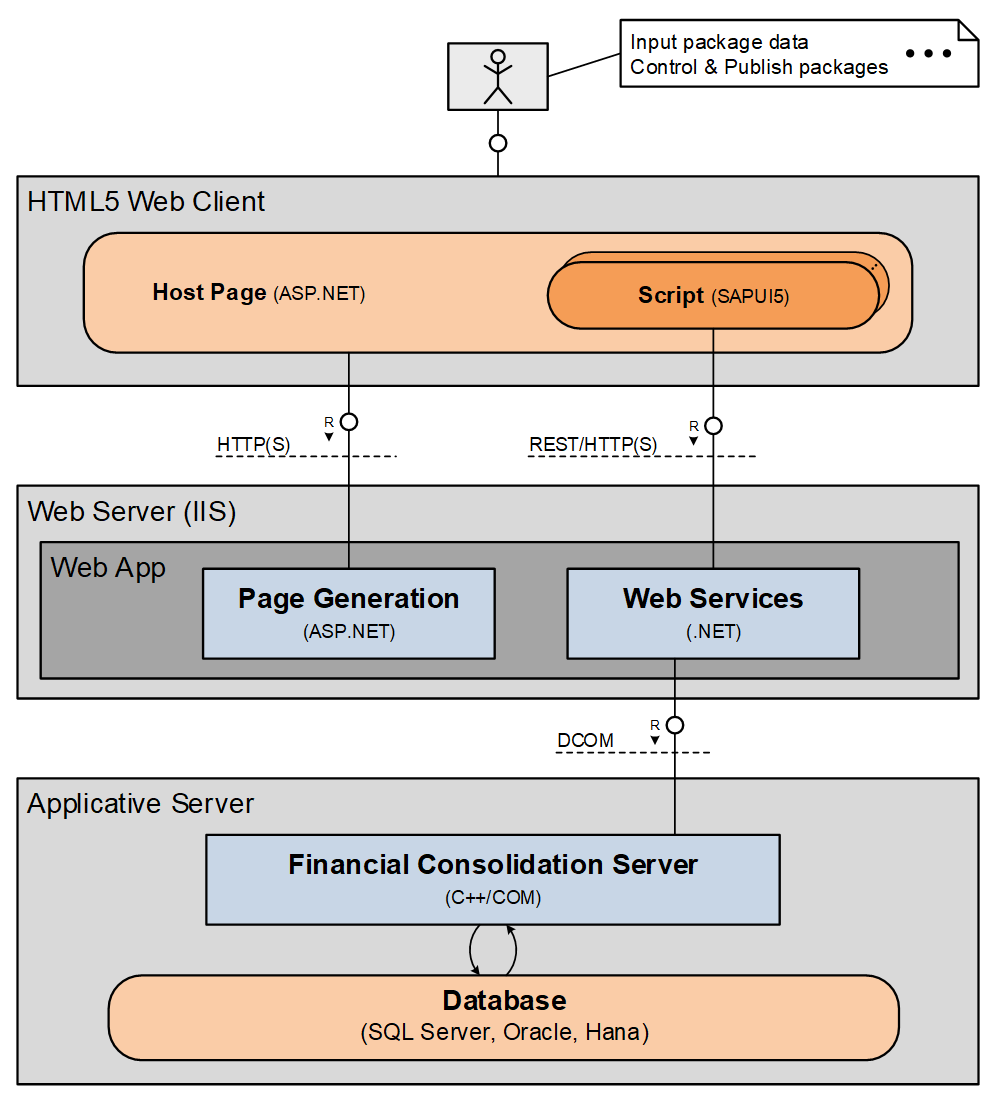
\includegraphics[width=0.8\textwidth]{FC_HTML5_Architecture.png}
        \caption{Financial Consolidation HTML5 Web Client Architecture}
        \label{fig:FC_HTML5_Architecture_label}
    \end{figure}
    
    \par Le Client HTML5 Web utilise la technologie SAPUI5 et fonctionne sur IIS(\textit{Internet Information Services}), il communique avec le Web Serveur en appelant le REST Services écrits en C\#, ce dernier communique avec application serveur par DCOM afin de finir les traitements.
    
    \newpage
    \subsubsection{Méthodologie du travail - Agile}
    Le produit FC existe depuis presque 20 ans, à l'époque, l'équipe FC avait travaillé avec les méthodes comme \textit{Modèle en cascade}, \textit{Cycle en V} comme la figure indique ci-dessous : 
    
    \begin{figure}[H]
       	\centering
    	\begin{subfigure}[b]{.4\textwidth}
    		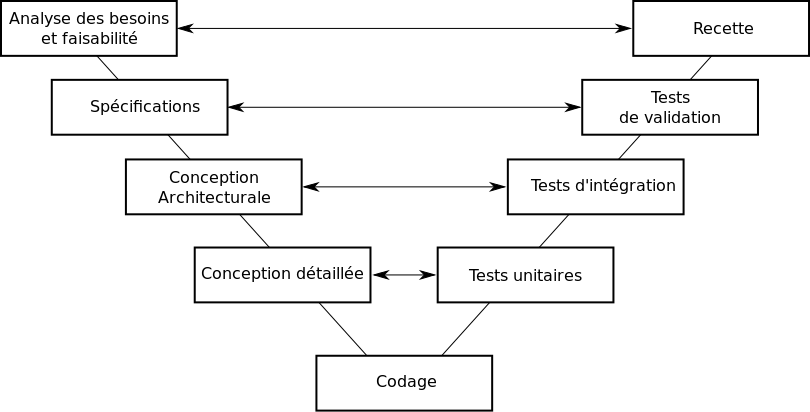
\includegraphics[width=\textwidth]{cycle_en_v.png}
    	\end{subfigure}
    	\begin{subfigure}[b]{.59\textwidth}
    		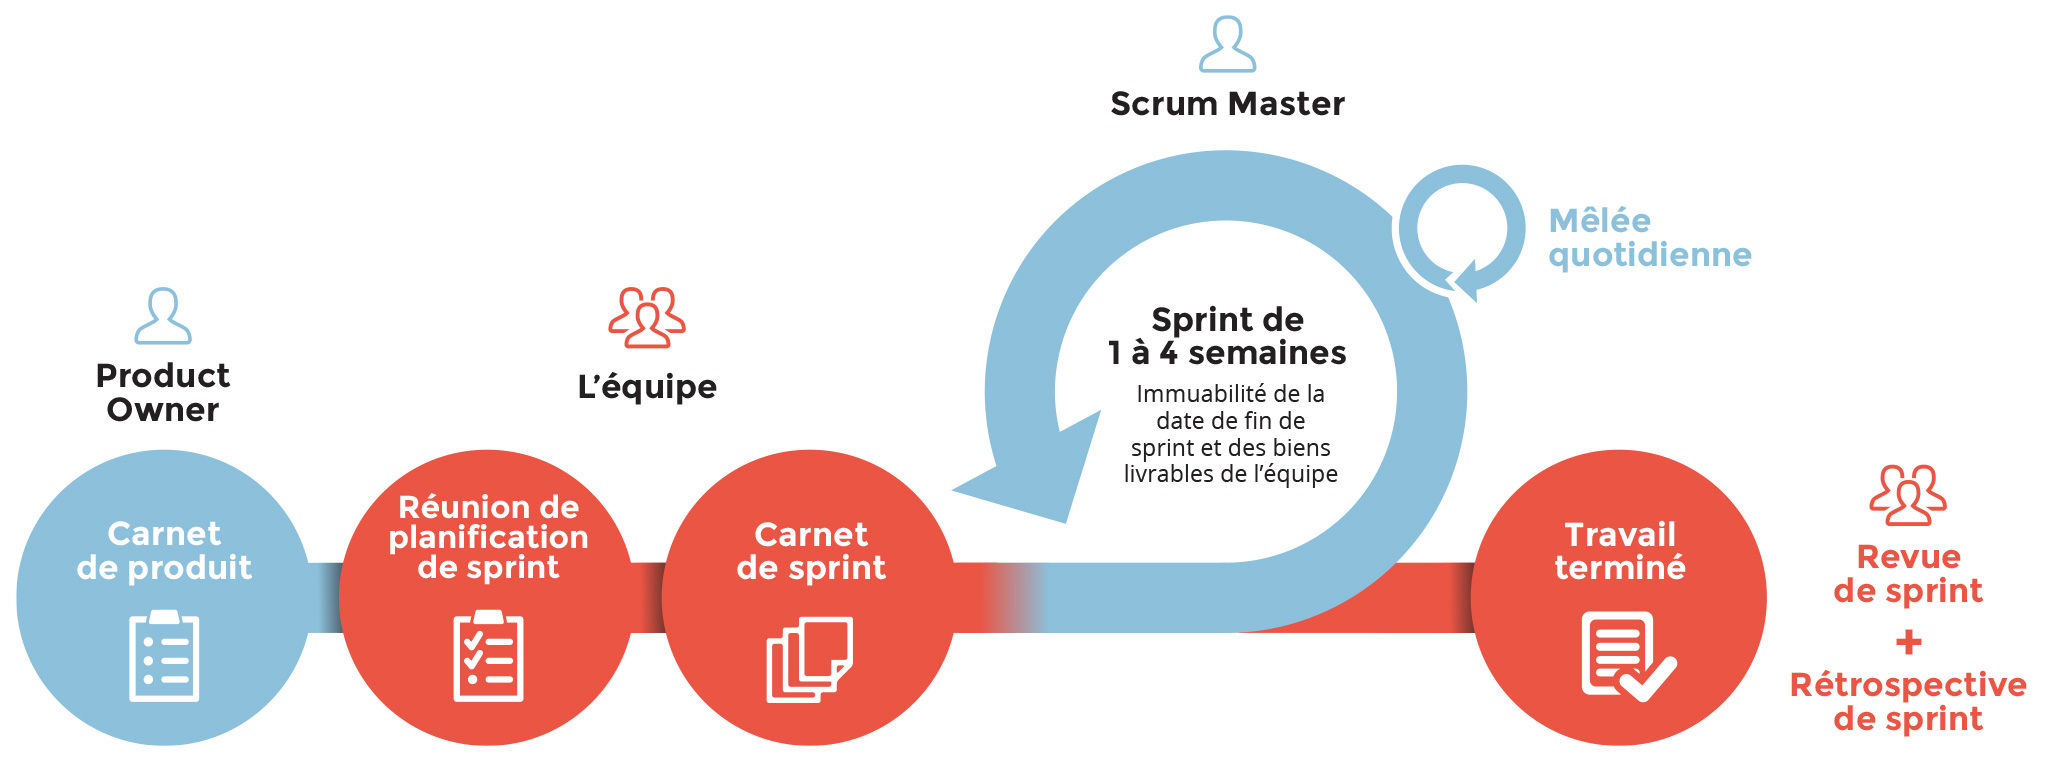
\includegraphics[width=\textwidth]{scrum.jpg}
    	\end{subfigure}
    	
    	\caption{Cycle en V vs Agile}
    	\label{fig: cycle_en_v}
    \end{figure}
    La méthode de cycle en V sépare les testeur et les développeur, cette méthode propose de retravailler par exemple la conception détaillée si les tests unitaires ne se valident pas ou de retravailler les spécifications si les tests de validation ne passent pas, contrairement, cette méthode ne convient pas beaucoup au besoin, elle prend beaucoup de temps à retravailler et faire la régression. Avec ces inconvénients de cycle en V et l'évolution de méthodologie de gestion du projet, SAP a demandé à l'équipe FC de travailler avec la méthode Agile, qui est s'adapte très bien aux besoins du projet FC. 
    
    \par Nous avons un tableau de mission collé sur mur qui indique l'avancement de chaque mission comme suivant : 
    \begin{figure}[H]
        \centering
        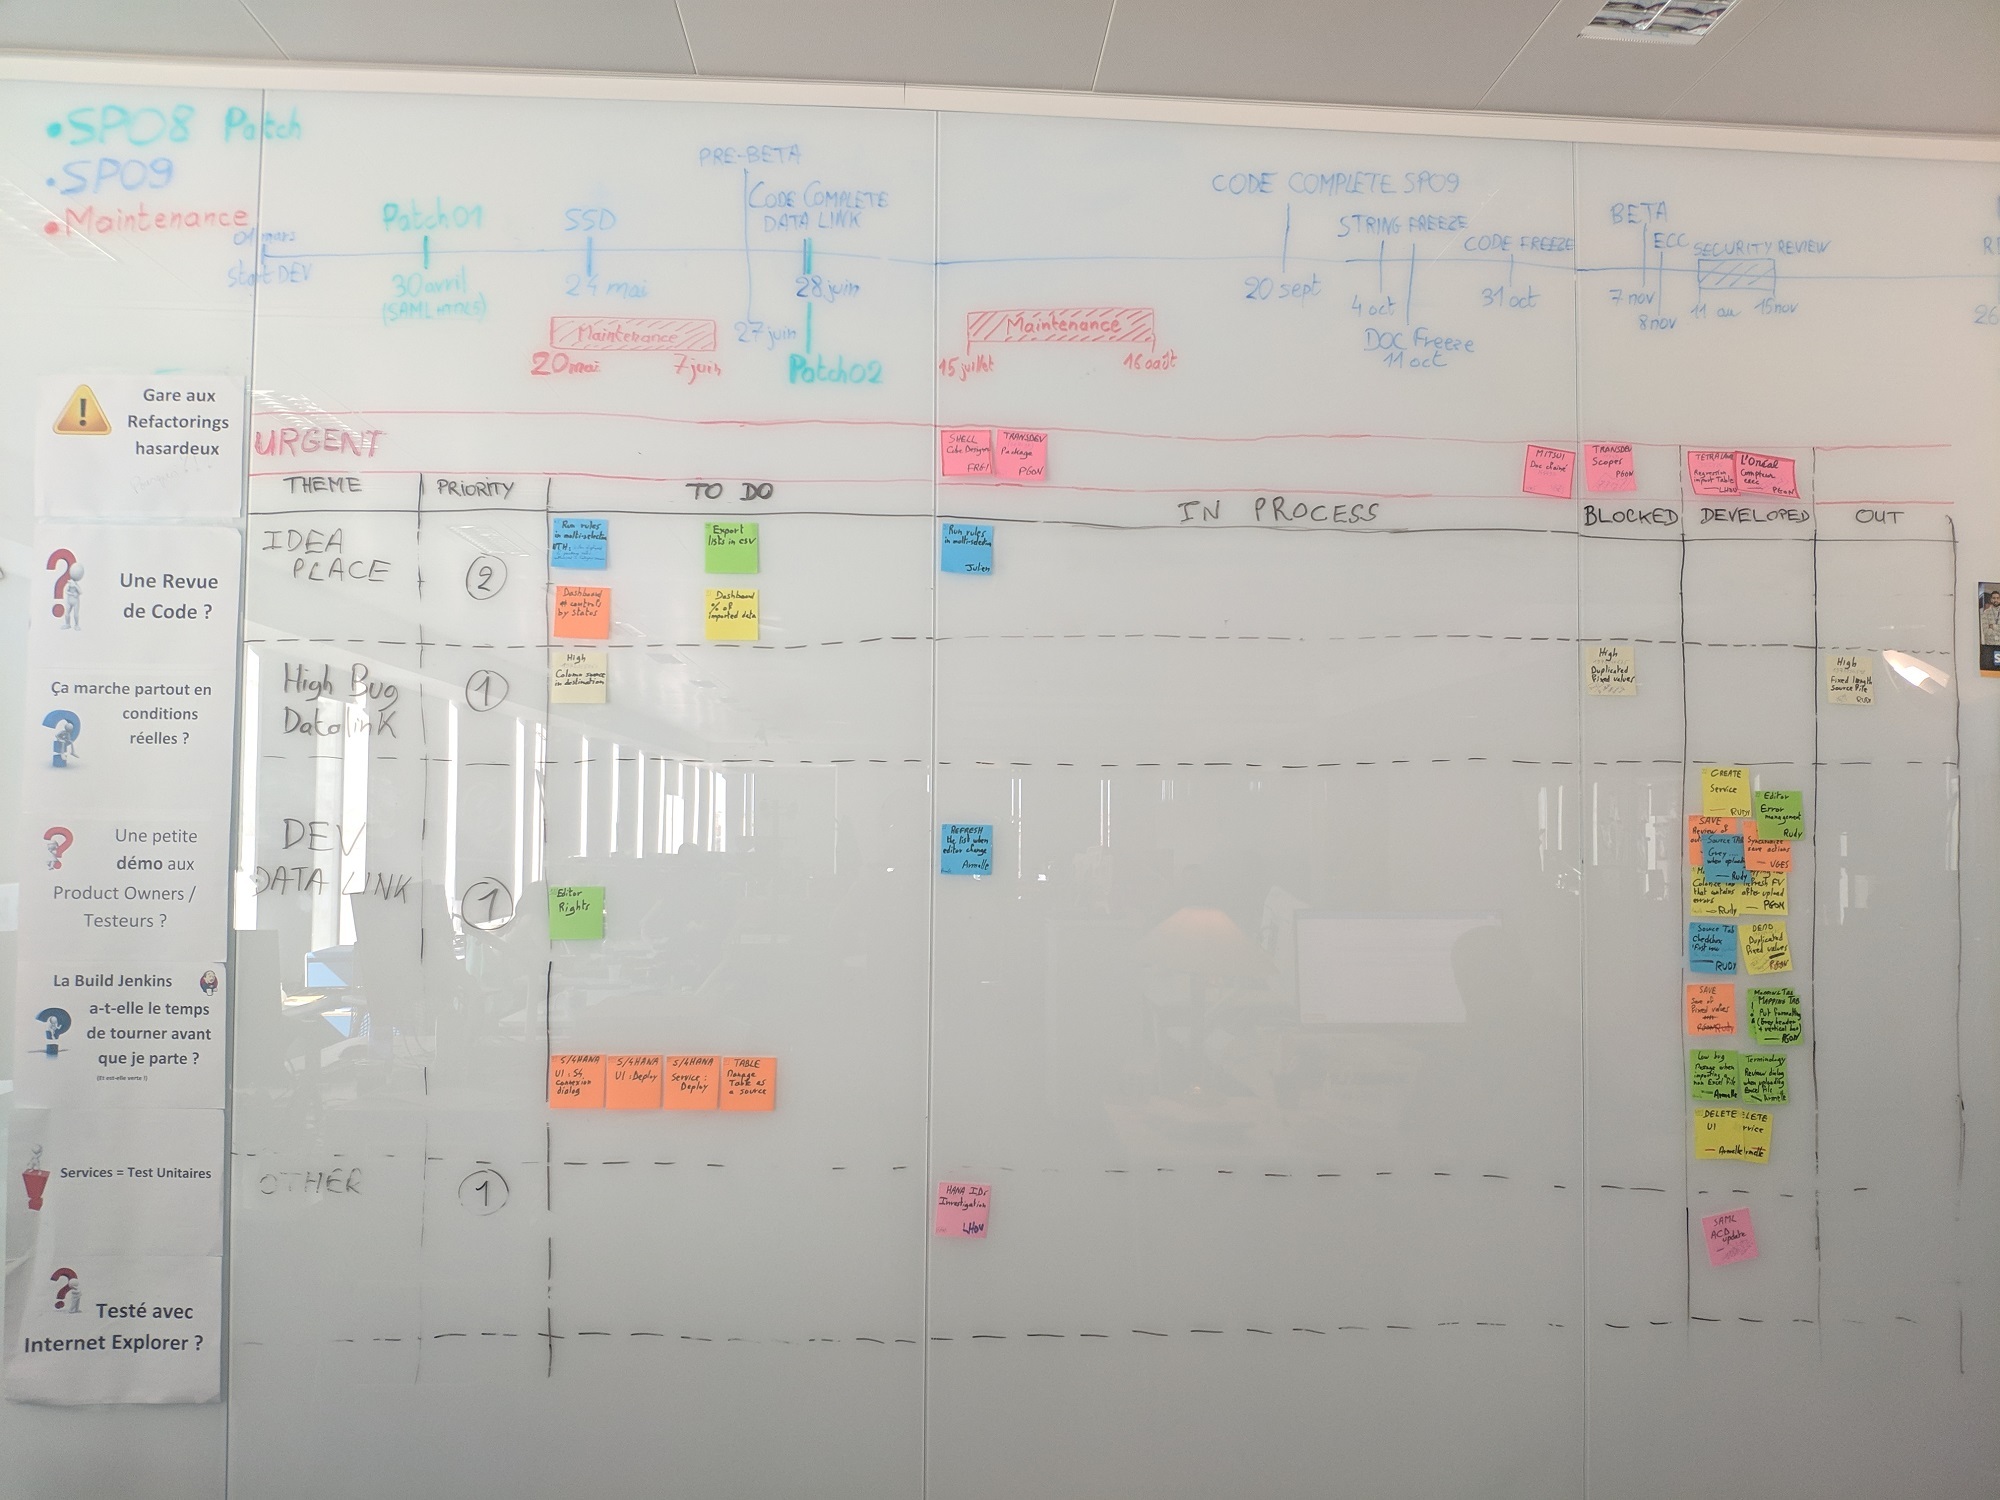
\includegraphics[width=0.9\textwidth]{scrum_tachTable.jpg}
        \caption{Scrum - Table des tâches}
        \label{fig:scrum_figure}
    \end{figure}
    \par Chaque jour pendant 13h40 et 14h00, notre Scrum Master Thierry GOOSSELIN organise une "Stand-up" réunion, avec \textit{Skype for Business} pour les collègues qui sone en télétrail, dans cette réunion, tous les membres d'équipe participent et restent debout au cours de laquelle chacun répond principalement à 3 questions : 
    \begin{itemize}[label=\textbullet]
        \item Qu'est ce que j'ai terminé depuis la dernière réunion ?
        \item Qu'est ce que j'aurai terminé d'ici la prochaine réunion ?
        \item Quels obstacles me retardent ?
    \end{itemize}
    
    \par Et pour chaque remonte du code importante, on a nos propres règles à respecter : 
    \begin{itemize}[label=\textbullet]
        \item Est-ce que j'ai fait une revue de code ?
        \item Ça marche partout en condition réelles ?
        \item Une petite aux Product Owners / Testeurs ?
        \item La Build Jenkins a-t-elle le temps de tourner avant que je parte ?
        \item Testé avec Internet Explorer ?
    \end{itemize}

    \subsubsection{Build et Livraison, Maintenance et Update}
    L'équipe FC a une organisation robuste pour la maintenance et mise à jour des produits. Pour chaque version de Financial Consolidation, il y a plusieurs SP (\textit{Support Package}), chaque SP a plusieurs Patch, on livre un nouveau SP environ chaque 9 mois qui contient des nouvelles fonctionnalités et des Bugs fixés, on livre un nouveau patch environ chaque mois qui ne contient que des Bugx fixés.
    \begin{figure}[H]
        \centering
        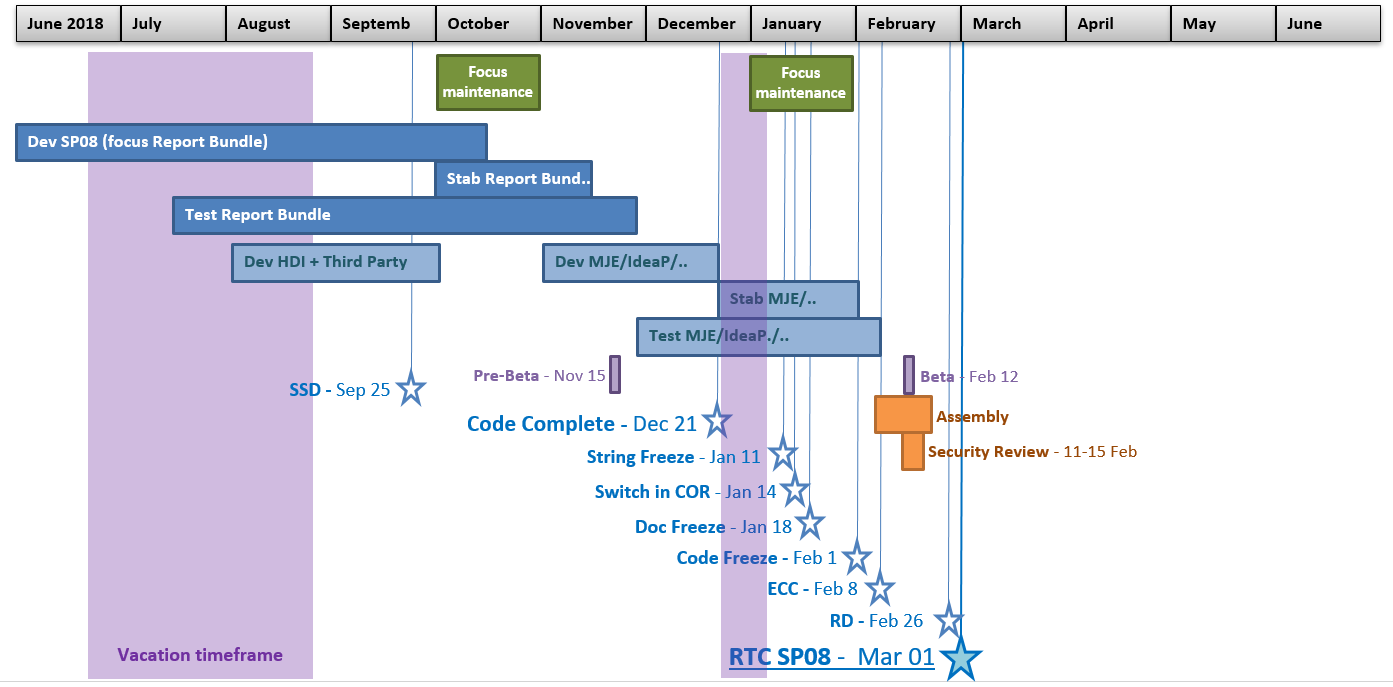
\includegraphics[width=\textwidth]{plan_SP.png}
        \caption{Time Line de Support Package}
        \label{fig:tileLine_sp}
    \end{figure}
    \par Quand on reçoit un bug envoyé par client,  en raison de travailler avec la méthodologie d'Agile, chaque développeur d'équipe peut prendre ce bug, ce fixe d'un bug va livrer au client dans le prochain patch. Dans l'image ci-dessous, on peut voir que pour le SP07, nous avons livré 6 patch en total.
    
    \begin{figure}[H]
        \centering
        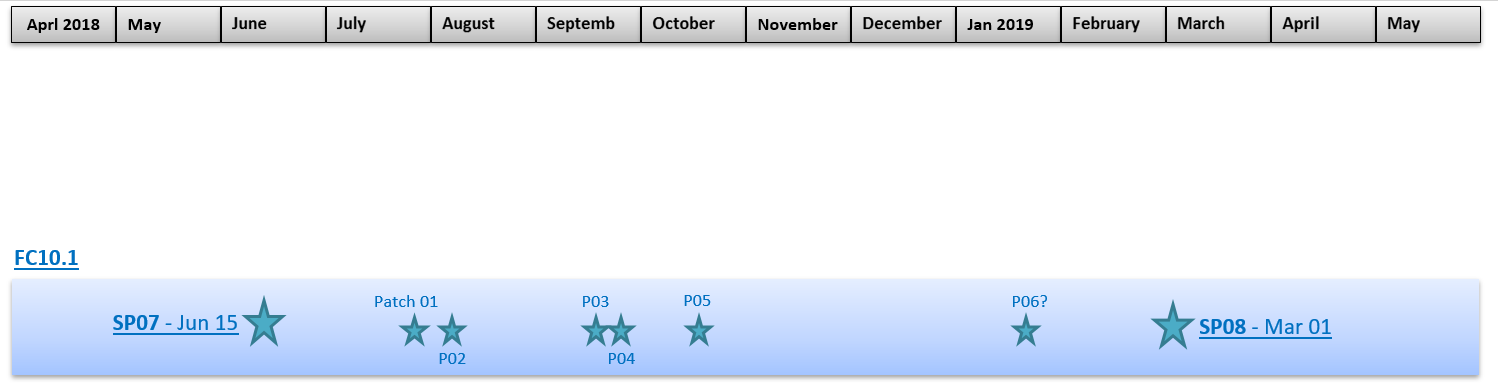
\includegraphics[width=.9\textwidth]{timeLine_patch.png}
        \caption{Time Line de Patch}
        \label{fig:timeLine_Path}
    \end{figure}
    \paragraph{Cycle de Build - Test - Release}
    \par Le produit FC est développé et délivré en mode pipeline.
    \begin{itemize}[label=\textbullet]
    	\item Afin de mieux organiser le développement du produit, l'équipe FC a décidé de soumettre les codes sur 3 branches : 
    	\begin{enumerate}
    		\item \textbf{Core} : La branche qui contient toutes les fonctionnalités et les nouvelles fonctionnalités du produit FC.
    		\item \textbf{PI} : La branche qui contient les fonctionnalités que l'équipe veut livrer au client, \textbf{\textit{c'est sur cette branche que l'équipe Test va faire les tests}}, et les développeurs corrige les bugs.
    		\item \textbf{Rel} : La branche qui va être livré et installé directement sur le coté client après la validation des tests.
    	\end{enumerate}
        \item Le Build de FC est fait sur ces 3 branches ci-dessus, il se déclenche à chaque nuit, ce build va donner à lendemain un résultat qui est coloré en rouge ou en vert. Rouge veut dire qu'il y avait une erreur sur le build ou des bugs sur les codes, on doit attendre la correction d'erreur et rebuild du soir prochain; vert veut dire que le build marche très bien, l'équipe Test peut récupérer et faire les test. Chaque build prend plus de 6 heures.
        \item Après le build, l'équipe Test va faire les tests manuel et test automatisé, nous faisons souvent les tests manuels sur les nouvelles fonctionnalités, les tests automatisés sur les non-régression fonctionnalités. Cet étape prend pas mal de temps et potentiellement trouver des bugs, les bugs viennent du développement sur les nouvelles fonctionnalités, ou les non-régression après le développement des nouvelles fonctionnalités, si on ne trouve pas de bug, on peut livrer le produit sur la branche \textit{Rel}.
        \item Si le test trouve des bugs, nos développeurs vont les fixer et remonter les codes pour le prochain build. 
    \end{itemize}
    \begin{figure}[H]
        \centering
        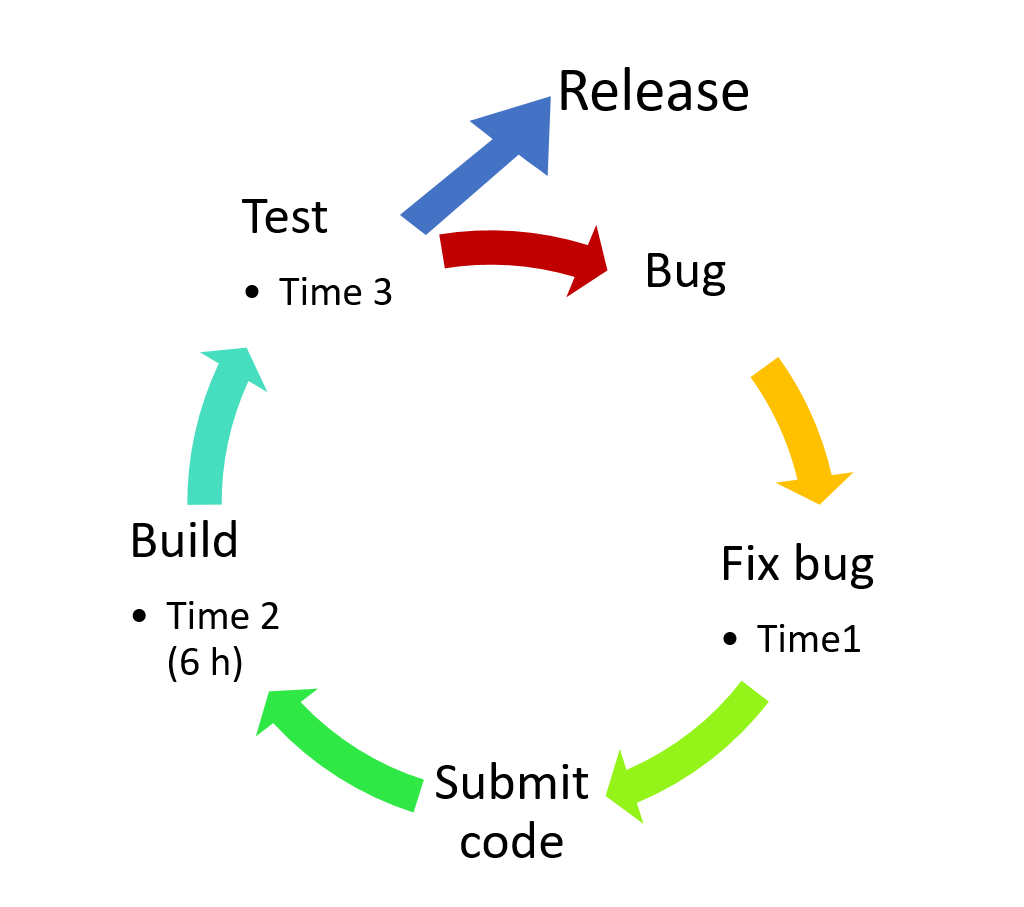
\includegraphics[width=\textwidth]{cycle_build_release.png}
        \caption{Cycle de Maintenance : Build et Release}
        \label{fig:cycle_maintenance_release_build}
    \end{figure}
    
    
%%%%%%%%%%%%%%%%%%%%%%%%%%%%%%%%%%%%%%%%%%%%%%%%%%%%%%%%%
\subsection{Client HTML5 : Test régression et Test non-régression}
	Le développement du produit amène deux théorie de test : Test de régression et Test de non-régression. Un test de régression est un ensemble de tests d'un programme préalablement testé, après une modification, pour s'assurer que des défauts n'ont pas été introduits ou découverts dans des parties non modifiées du logiciel. Test de non-régression est un le même test avec test de régression mais sans modification pour assurer la qualité de produit.

    \subsubsection{Comparaison Test Manuel et Test Automatisé}
    Grâce aux technologies utilisés pour le développement de Client HTML5, nous pouvons automatiser certains tests fonctionnels en manipulant les XPath (\textit{XML Path Langage}) de contrôle sur navigateur. Pour le choix de faire test manuel ou test automatisé, les comparaisons sont dans le tableau ci-dessous. Finalement, l'équipe a choisi ces deux méthodes avec test automatisé couvre 50\%-60\% de fonctionnalité, les restes sont les tests manuels.
    \begin{table}[H]
        \centering
        \begin{tabular}{|c|m{5cm}|m{5cm}|}
            \hline
             & \Large{\textbf{Avantages}} & \Large{\textbf{Désavantages}}\\
             \hline
             \Large{\textbf{Test Manuel}}   &
                % Avantage de test manuel
                \begin{itemize}[label=\textbullet]
                    \item Permet de trouver les erreurs ne sont pas dans le scénario qui peut potentiellement gênant pour le produit.
                    \item Permet de test le UX.
                    \item Très utile pour faire les tests régressions.
                \end{itemize}
                                    &
                \begin{itemize}[label=\textbullet]
                    \item Facile d'être fatigué faces aux scénarios \textit{répétés}, perdre de temps.
                \end{itemize}                    
                                    \\
             \hline
             \Large{\textbf{Test Automatisé}} & 
                 \begin{itemize}[label=\textbullet]
                     \item Scripts de test peuvent être réutilisés
                     \item Pas de fatigue, moins d'erreurs
                     \item Augmenter la couverture : plus de langue, plus de type de navigateur
                     \item Assurer la qualité du produit, détecte les régressions (une fonctionnalité ne marche pas après ajouter les nouvelles features)
                     \item Très utile pour faire les tests de non-régression sur les fonctionnalités existantes.
                 \end{itemize}
                                     & 
                \begin{itemize}[label=\textbullet]
                    \item Dépendance d'environnement, par fois ne marche pas même si le Test Robot marche bien sur la machine de développeur
                    \item Test Robot fait ce que les codes demandes, ignore les erreurs visuels.
                    \item Stabilité faible, une petite modification UI d'application peut bloquer le Test.
                \end{itemize}
                                     \\
             \hline
        \end{tabular}
        \caption{Comparaison entre Test Manuel et Test Automatisé}
        \label{tab:TestManuel_vs_TestAuto_label}
    \end{table}

	\subsubsection{Pourquoi Test Automatisé est demandé ?}
	Après la discussion de la comparaison entre Test Manuel et Test Automatisé, et le cycle de Build et Release dans les parties précédentes, on peut savoir que Test Automatisé est plus pratique pour faire des tests de non-régression sur les fonctionnalités existantes parce qu'il peut répéter le scénario de test facilement.
	
	\par Dans le développement du produit, les QA(Quality Assurance) assurent la qualité du produit en testant les nouvelles fonctionnalités et en faisant des tests de non-régressions sur les fonctionnalités existantes. Avec cette raison, l'équipe avait décidé d'automatiser le plus nombreux de tests non-régressions possible, c'est dans ce cas le Test Automatisé est demandé comme un point important dans 

\subsubsection{Langages et Technologies utilisées pour réalisation de Test-Auto}
    Nous avons choisi d'utiliser SilkTest et Java pour développer le test-auto, les raisons de faire ce choix sont suivantes : 
    \begin{itemize}
        \item SilkTest est déjà utilisé par une autre équipe de SAP France avant le commence du projet test-auto, les expériences d'utilisations d'un autre équipe nous a aidé beaucoup.
        \item Le choix du langage Java a été de préférence du développeur pour commencer le projet test-auto.
    \end{itemize}
    
    \paragraph{SilkTest VS Selenium}
    Néamoins SilkTest est actuellement utilisé pour le test-auto de FC, l'équipe de Test a décidé d'utiliser Selenium comme outil de test-auto pour le projet à l'avenir, les raisons sont dans le tableau ci-dessous : 
    
    \begin{table}[H]
        \centering
        \begin{tabular}{|r|m{5cm}|m{5cm}|}
        \hline
        & \Large{\textbf{Silk Test}} & \Large{\textbf{Selenium}} \\
        \hline
            Prix & Acheter Licence & Open source - Gratuit \\
        \hline
            Test Système & Microsoft Windows & Cross-plateform : Windows, Linux, Mac\\
        \hline 
            Applications à tester & Web, Modbile, Windows C$\backslash$S & Web application\\
        \hline
            Développement langage supporté & C\#, Java & Java, C\#, Perl, Python, JavaScript, Ruby, PHP\\
        \hline
        \end{tabular}
        \caption{SilkTest VS Selenium}
        \label{tab:Silk_vs_Selenium_label}
    \end{table}
%\subsubsection{Procédure de test automatisé sur les machines virtuelles}
\newpage
\subsection{Test d'impression}
    \subsubsection{Analyse du problème et Etat de l'Art}
    Dans le cadre de test fonctionnel du FC, nous avons eu besoin de tester s'il la fonctionnalité d'impression de rapport dans l'application marche bien, c'est à dire pour le même rapport, l'impression donne toujours le même fichier pdf entre différentes versions.
    
    \par Avant je suis arrivé, pour ce test, nous avons fait manuellement, c'est à dire que nous imprimons ces fichiers pdf et vérifié la différence entre ces pdf, c'est très fatiguant pour les testeurs, en plus, nous en tant que humains, nous ne pouvons pas vérifier les petites différences, par exemple la différence de police des lettres, la différence entre lettre \textbf{'o'} et \textbf{'0'}.
    \begin{figure}[H]
        \centering
        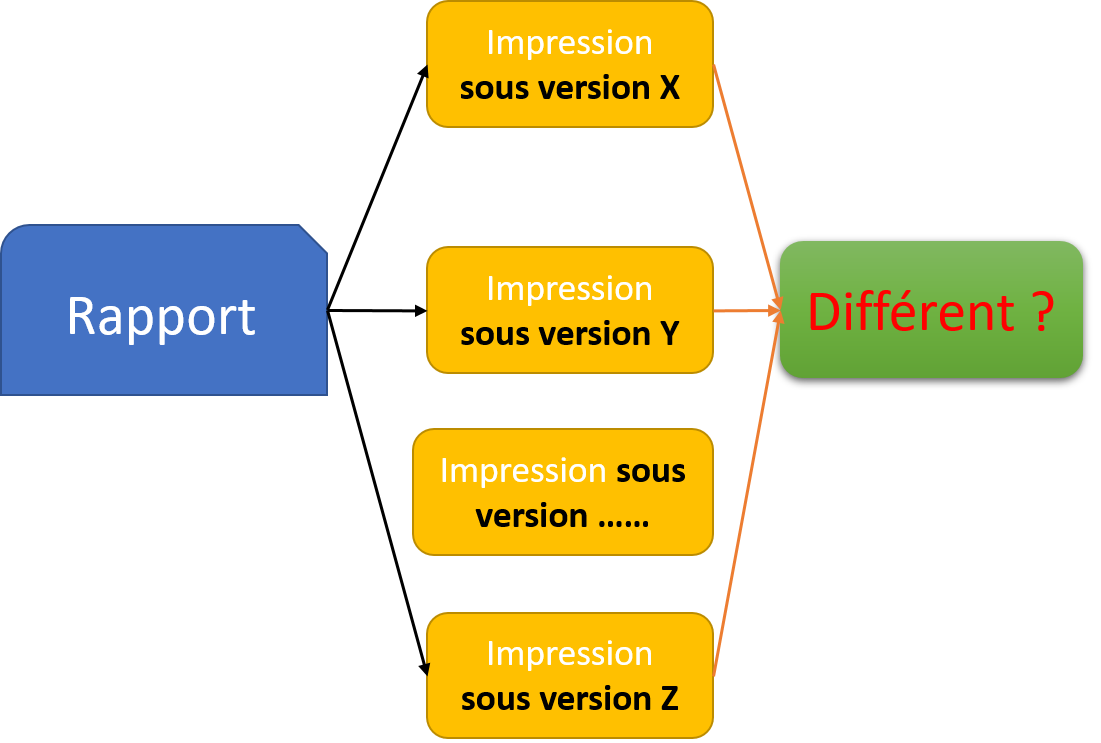
\includegraphics[width=\textwidth]{problematique_print.png}
        \caption{Problématique du test d'impression }
        \label{fig:prolematique_TestPrint_label}
    \end{figure}
    
    \subsubsection{Comparaison les pdf avec checksum ou pixel par pixel}
    \par Dans cette condition, ça nous fait un besoin de comparer la différence entre deux fichier pdf par machine. La façon la plus rapide est de générer une valeur de checksum (\textit{MD5, SHA-1, SH-2}, etc.) pour chaque pdf, puis on vérifier la différence entre ces deux valeurs, s'ils sont les mêmes, ça va dire que ces deux pdf sont les mêmes, sinon, ça va dire que les deux pdf sont différents. Mais la comparaison avec checksum ne peut pas indiquer la position où il y a des différences entre 2 fichiers. Pour cette raison, j'ai décidé de faire une comparaison de pixel par pixel, qui est plus précisé et plus lisible par les humains. 
    
    \begin{table}[H]
        \centering
        \begin{tabular}{|r|m{4cm}|m{4cm}|}
            \hline
            &   \Large{\textbf{Avantages}} & \Large{\textbf{Désavantages}}\\
            \hline
            \textbf{Checksum comparaison} & Rapide & Ne peut pas indiquer les positions de différences  \\
            \hline
             \textbf{Pixel par Pixel comparaison} & Peut indiquer les positions de différences  & Compiliquer à programmer, traitement lent \\
             \hline
        \end{tabular}
        \caption{Checksum comparaison VS Pixel par Pixel comparaison}
        \label{tab:pixel_vs_checksum_label}
    \end{table}
    \par Puisque deux fichier pdf n'est jamais le même, donc nous pouvons aussi définir une cohérence de différence, on dit qu'il y a la différence entre deux pdf si le taux de différence est supérieur à la cohérence (0,3\% par exemple).
    
    \par Avec les conditions et raisons ci-dessus, l'équipe de test m'a donné la tâche d'automatiser le test d'impression et l'intégrer dans le processus de test-auto sur Jenkins comme la mission principale de mon alternance.

\newpage
%%%%%%%%%%%%%%%%%%%%%%%%%%%%%%%%%%%%%%%%%%%%%%%%%%%%%%%%%%%%%%%%%%%%%%%%%
\section{Travail réalisé}
\subsection{Schéma global}

    \subsubsection{Architecture de Test-Auto}
    La mission de mon alternance est d'automatiser les scénarios de test automatisé, quand je suis arrivé, l'architecture de Test-Auto est déjà conçu et réalisé. Nous avons utilisé les machines virtuelles, Jenkins slave, et Perforce afin de lancer les tests et héberger les bases de données que ce dernier aura besoin pendant le tests. les principes de test automatisé sont suivant : 
    \begin{itemize}
        \item 3 types de machines virtuelles : machine qui contient la base de donnée utilisé par FC; machine qui contient les ressources de référence de tests, cet machine va faire une copie de base de donnée celle de précédente; machine virtuelle avec Jenkins slave, produit FC et Junit installés, c'est dans cette machine qu'on lancer les tests.
        \item Une machine virtuelle contient les logs de tous les test-auto, et ces logs vont afficher dans un fichier Excel qui est plus lisible au lieu d'être en format .txt.
        \item Les test-auto codes sources de \textit{JUnit} manipulés par Perforce, ces codes vont être exécuter dans une ou toutes les hosts machines selon la configuration.
        \item Un Jenkins master qui va lancer tous les tests et bien générer les résultats de test.
    \end{itemize}
    \begin{figure}[H]
        \centering
        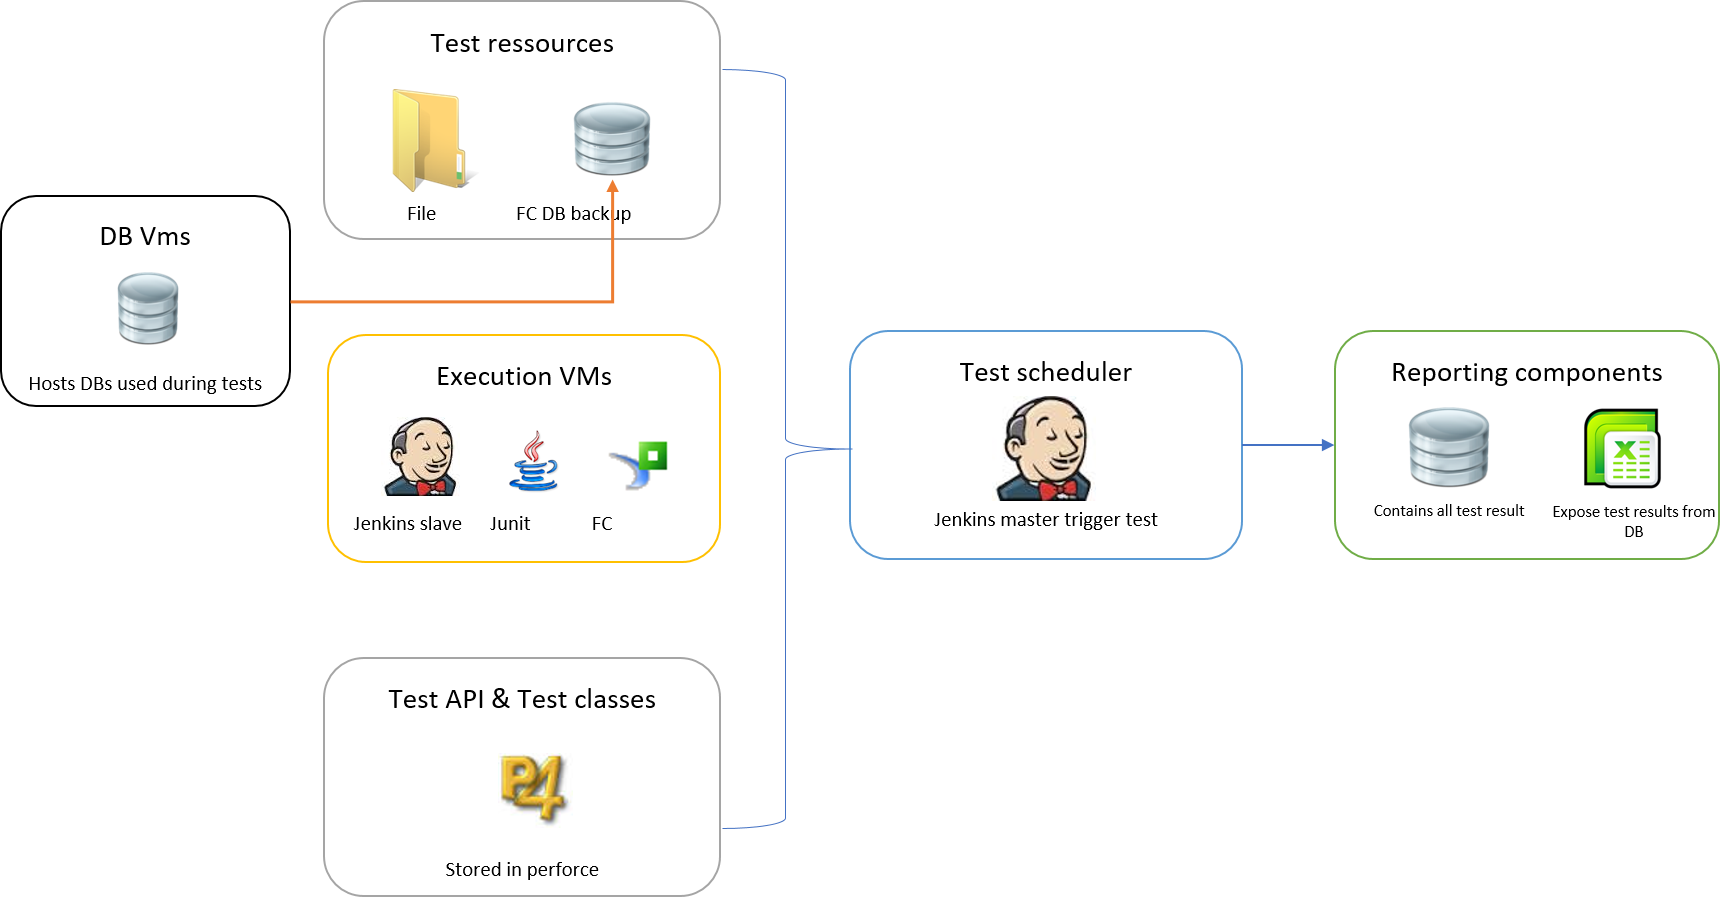
\includegraphics[width=.85\textwidth]{TestAuto_architecture.png}
        \caption{Architecture de Test Automatisé}
        \label{fig:Architec_testAuto}
    \end{figure}

\subsection{Développements Réalisés}
 
    \subsubsection{Réalisation les scénarios des opérations sur les packages}
    Quand je suis arrivé, l'équipe Test m'a donné une tâche de réalisation les test-auto pour les opérations de packages de consolidation financière pour me familiariser avec les outils, l'environnement de travail. Il y avait 3 scénarios en totale et je l'ai finis pendant environ 10 jours, cette tâche me permet de bien comprendre l'architecture de Test-auto présentée dans la partie précédente, me permet de parcourir les codes existants, de comprendre le mécanisme comment sauvegarder des logs de Test, de comment déclencher une application par exemple navigateur \textit{IE} et \textit{Google Chrome} sous exploitation Windows avec SilkTest, de comment manipuler les contrôles d'une application avec XPath, etc.
    
    \par Après cette tâche, je suis demandé de concentré sur la tâche principale - test-auto d'impression, en réalisant les petites tâches peuvent être arriver de temps en temps. 
    \subsubsection{Comparaison entre deux PDF}
    
    \begin{figure}[H]
        \centering
        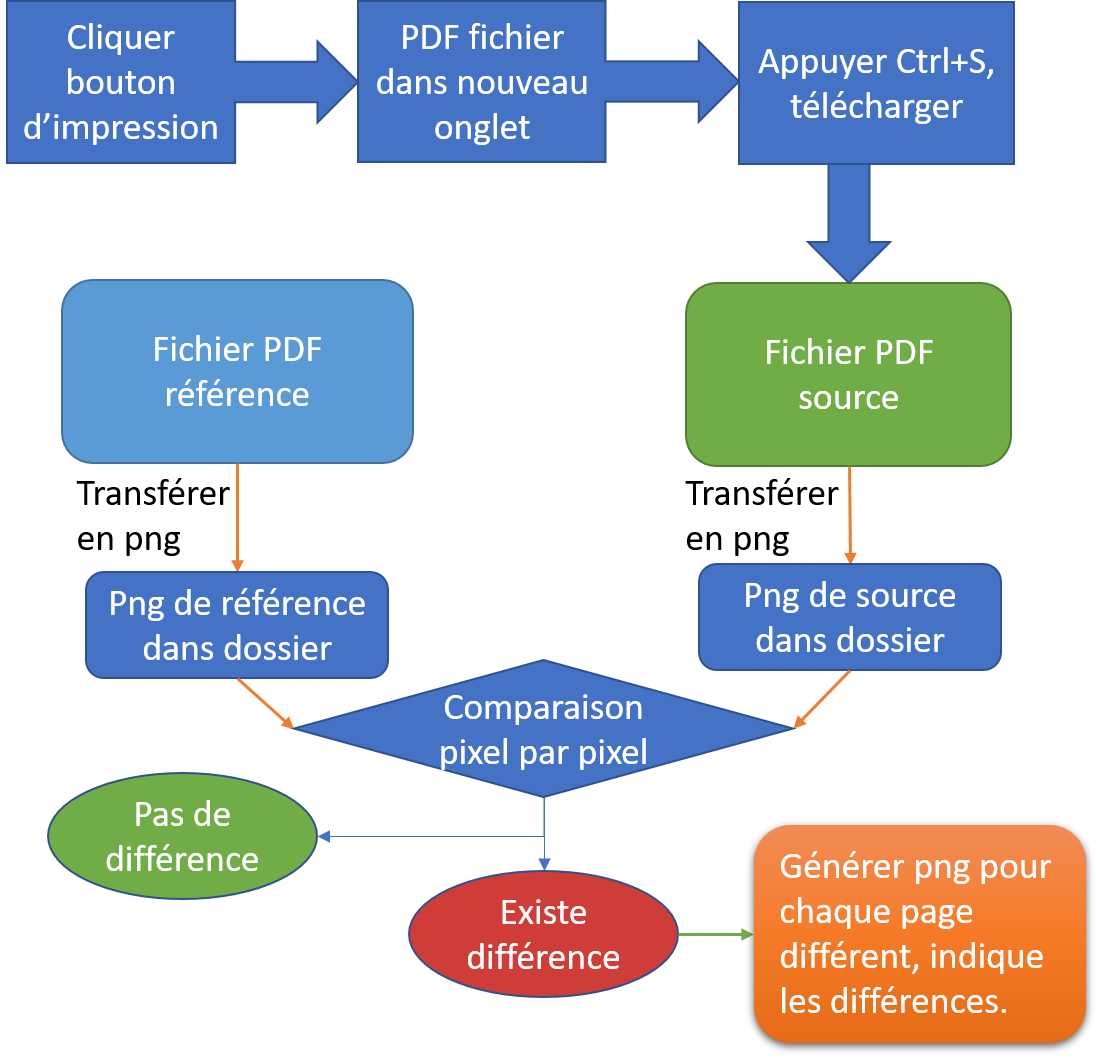
\includegraphics[width=.8\textwidth]{process_compar_pdf.png}
        \caption{Processus de comparaison de deux rapports}
        \label{fig:proc_compar_report_label}
    \end{figure}
    Dans l'application, le bouton d'impression d'un rapport ou plusieurs rapports résulte d'un téléchargement à partir de navigateur. Pour le téléchargement de plusieurs rapport, je vais discuter dans la partie prochaine. Pour la comparaison entre deux fichiers pdf, le processus que j'ai conçu est ci-dessous : 
    \begin{enumerate}[label=\arabic*)]
        \item Le rapport de référence est déjà fourni par le testeur, navigateur est préconfiguré pour que le téléchargment de pdf s'ouvre dans un nouvel onglet.
        \item Cliquer sur le bouton d'impression dans l'application FC, le rapport pdf s'ouvre dans le nouvel onglet, mettre focus sur le nouveau onglet.
        \item Appuyer \textbf{Ctrl+S} sur le nouvel onglet, il y a une dialogue de téléchargement apparaître, télécharger le fichier avec le nom fournis.
        \item Pour chaque page de fichier pdf de référence et de source, générer une image en format png, les mettre dans un nouveau dossier créé dans le même répertoire du rapport avec le nom "\textit{png\_Nom\_du\_pdf}".
        \item Comparer les images dans les deux dossiers, s'il n'y a pas de différence, on passe à la prochaine étape; sinon, générer les images en noir et blanc comme ci-dessous indique les différences, ensuite rejeter une exception qui va être écrit dans log et arrêter le test de scénario problématique.
        \begin{figure}[H]
            \centering
            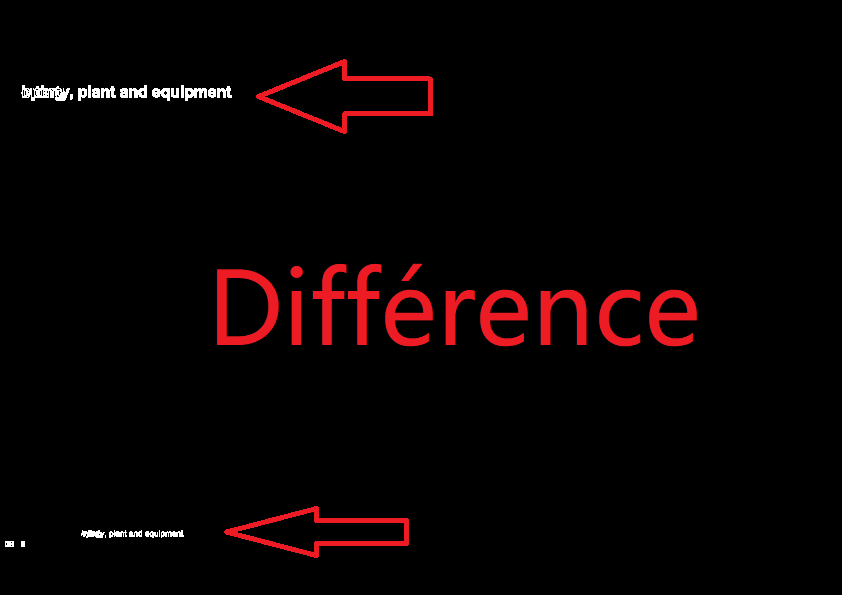
\includegraphics[width=0.5\textwidth]{png_difference.png}
            \caption{Exemple de différence dans un pdf}
            \label{fig:exemple_pdf_diff_label}
        \end{figure}
    \end{enumerate}
    
    Parce qu'une autre groupe de SAP France a déjà fait des traitements similaires, donc nous avons récupéré leurs codes de comparaison entre deux pdf, j'ai tout compris ce que leurs codes ont fait et je les ai adapté à notre projet. Dans leurs codes, un point très bien et je peux toujours me servir est leurs codes utilisent deux threads différentes pour traiter le pdf de référence et le pdf de ressource en parallèle, cette méthodologie a beaucoup amélioré l'efficacité, la partie d'annexe \textbf{\ref{appendix: multi-thread_compare_pdf}} contient les codes sources de cette réalisation. 
    
    \subsubsection{Télécharger et décompresser un zip}
    Pour certains scénarios de tests, on demande de télécharger un fichier zip, le nom de ce zip contient un GUID \textit{(globally unique identifier)} préfix, le nombre des fichiers pdf et les noms sont déjà connus, ils ont aussi le même préfix pour leurs noms. Pour ces  fichiers pdf dedans, on demander de les renommer avec les noms donnés selon l'ordre de choix de rapport dans FC.
    
    \par Pour cela, J'utilise une bibliothèque standard de Java  \textit{java.util.zip.ZipEntry} et  \textit{java.util.zip.ZipInputStream} afin de décompresser le zip, ensuite, j'ai utilisé lambda expression de classer les fichiers selon leurs temps de création, puis le renommer.
    
    \subsubsection{Comparaison les pdf dans deux répertoires avec \textbf{\textit{Lambda Expression}}}
    Après avoir fini la tâche dans la partie précédente, nous avons des nouveaux besoins : on ne sait pas le nom ou le préfix de nom des fichiers pdf dans le zip, ni le nombre des pdfs dans le zip. Autrement dit, ces besoins nous demandent de faire la comparaison entre tous les fichiers pdf ont le même nom dans deux répertoires. 
    
    \par Pour la comparaison, on peut appeler la méthode qu'on a développé, pour comparaison de tous les fichiers pdf, on peut parcourir le répertoire et faire la comparaison dans plusieurs boucle \textit{\textbf{for}}, mais cette méthode demande trop de complexité. 
    
    \par Après avoir réfléchi, j'avais trouvé qu'on peut faire le parcourir de répertoire avec \textit{\textbf{Lambda Expression}}, qui est une très importante mise à jour depuis la création du langage Java, et il est beaucoup utilisé par les autres langages, c'est très "en mode" dans le monde de programmation aujourd'hui. Les codes utilisent \textbf{\textit{Lambda Expression}} sont élégants et ne prennent pas beaucoup de place, pour la comparaison entre deux répertoire, il ne m'a pris que 10 lignes de code. Dans la partie d'annexe \textbf{\ref{appendix:lambda_compare_towFolder}} contient les codes sources de cette réalisation. 
    
    \par \textit{\textbf{Lambda Expression}} est une manière élégante de penser pour la programmation ! 
    
    
    \subsubsection{Outils utilisés}
    Pour réaliser les travaux parlés ci-dessus, nous utilisons les outils ci-dessous : 
    \paragraph{Gestion du code - PERFORCE}
    Pour la gestion de version du code, nous utilisons Perforce.
    \begin{figure}[H]
    	\flushleft
    	
\includegraphics[width=.3\textwidth]{Perforce_Logo.jpg}
    	\label{fig:Perforce_Logo}
    \end{figure}
    \par Perforce est un outil de gestion de configuration utilisé dans le processus de développement logiciel, Perforce est un système de contrôle de version centralisé, c'est ici la différence avec les autres système de contrôle de version comme Git, Mercurial. Nous utilisons un des ces outils Helix Visual Client (P4V), Helix Visual Client (P4V) est une application de bureau qui permet d’accéder aux fichiers versionnés dans Helix Core via une interface graphique. Il comprend des outils permettant de fusionner et de visualiser l'évolution du code.
    \par Avec P4V, il est facile de personnaliser notre espace de travail afin de ne voir que les fichiers dont nous avons besoin. Nous pouvons travailler hors ligne et à distance. Et lorsque nous avons terminé, transférez facilement les modifications locales sur un serveur distant. 
    \par Nous pouvons :
    \begin{itemize}
    	\item Voir les changements de time-lapse et de révision. 
    	\item Obtenez un aperçu des métadonnées du projet.
    	\item Demander des révisions de code sur les modifications en attente.
    \end{itemize} 
    \par Dans notre équipe, chaque remonte du code est revue par l'autre développeur, pour moi, c'est mon encadrant technique Sébastien Coudray relit mes codes. 
    
    \paragraph{Édition du code - Eclipse}
    Avec la limite que le plugin Silk4J ne peut qu'installer sur Eclipse, l'équipe de test-auto a décidé d'utiliser Eclipse comme éditeur du code.
    \begin{figure}[H]
    	\flushleft
    	
\includegraphics[width=.3\textwidth]{Eclipse_logo.png}
    	\label{fig:eclipse_logo}
    \end{figure}
    
    \paragraph{Outil de Testauto : SilkTest - Silk4J}
    \par Silk Test est un outil de test de fonction automatisé et de régression des applications d'entreprise. Le plugin Silk4J installé sur Eclipse nous permettons de créer des tests fonctionnels avec la programmation en Java, avec la Java runtime librairie fournis par Silk4J, on peut lancer des JUnit test.
    \begin{figure}[H]
    	\flushleft
    	
\includegraphics[width=.3\textwidth]{silktest_logo.png}
    	\label{fig:silktest_logo}
    \end{figure}
    
    \par L'outil "Locator Spy" installé ensemble avec SilkTest nous permet de localiser les contrôles d'une application et afficher comme un \textbf{XPath} comme la figure ci-dessous, c'est un outil que je peux l'utiliser pour reconnaître le ID d'un contrôle puis l'utiliser dans mon code.
    \begin{figure}[H]
    	\flushleft
    	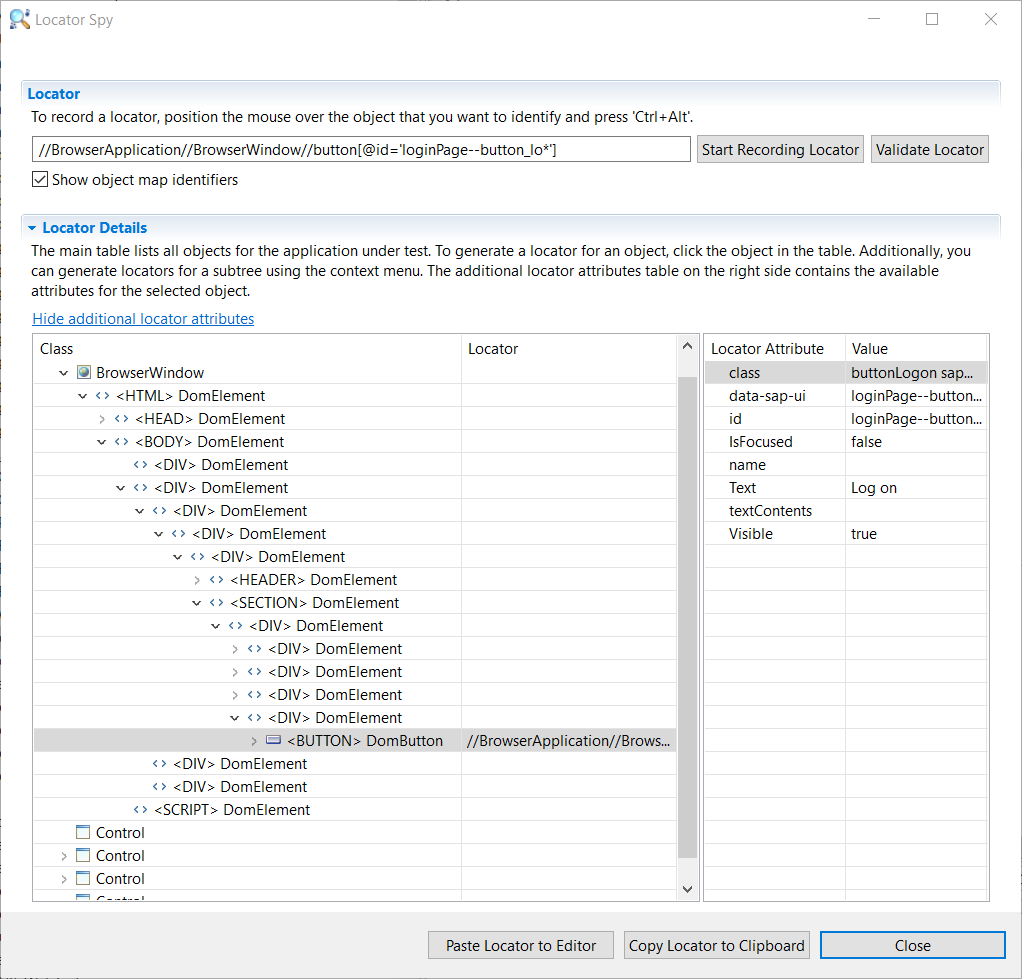
\includegraphics[width=.7\textwidth]{silk_locator_spy.PNG}
    	\label{fig:silk_locator_spy_label}
    \end{figure}
    
    \paragraph{Intégration continue - Jenkins + machines virtuelles}
    Afin d'automatiser le build et les tests fonctionnels, l'équipe FC a mis en service une Intégration Continu de build et de Test-auto avec Jenkins et plusieurs machines virtuelles. Nous pouvons se connecter aux ces machines virtuelles avec le client \textit{Remote Desktop Connection} sous Windows.
    \begin{figure}[H]
    	\flushleft 
    	\begin{subfigure}[b]{.35\textwidth}
    		
\includegraphics[width=\textwidth]{jenkins_logo.png}
    	\end{subfigure}
    	\begin{subfigure}[b]{.35\textwidth}
    		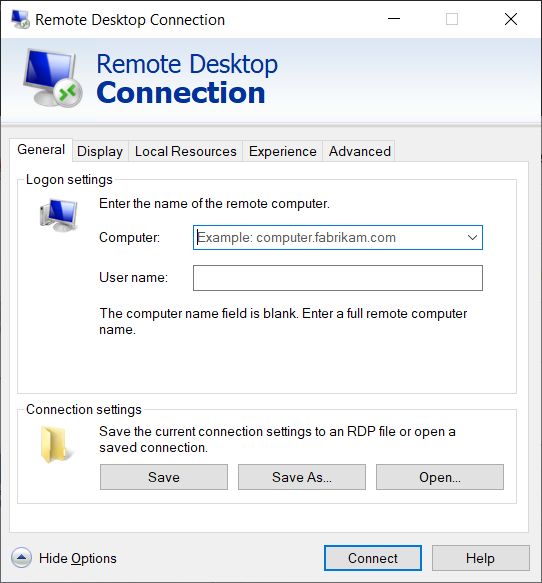
\includegraphics[width=\textwidth]{win_remote_desktop.PNG}
    	\end{subfigure}
    	\label{jenksin_+_win_remote_desktop_label}
    \end{figure}
    
    
    \paragraph{Partage de fichiers et d'informations - One Note + One Drive }
    Pour partager les fichiers et les informations nécessaires d'équipe, nous utilisons OneNote et OneDrive, OneNote pour sauvegarder les informations des projets : Notes pour chaque réunions, IP des machines virtuelles, liens des dossiers partagés, tâches de chaque personne avant prochaine réunion de revue, etc. OneDrive pour partager les documents.
    
    \begin{figure}[H]
    	\flushleft
    	\begin{subfigure}[b]{.2\textwidth}
    		
\includegraphics[width=\textwidth]{OneNoteLogo.png}
    	\end{subfigure}
    	\begin{subfigure}[b]{.2\textwidth}
    		
\includegraphics[width=\textwidth]{OneDriveLogo.png}
    	\end{subfigure}
    	\label{fig:oneNote_oneDrive_label}
    \end{figure}
    
    \paragraph{Communication interne - Skype for Business + Outlook}
    Pour communication interne, nous utilisons Skype for Business et Outlook.
    
    \par Skype for Business est un logiciel d'entreprise de messagerie instantanée développé par Microsoft, ce logiciel nous permet de se communiquer entre membre de l'équipe, il nous permet aussi d'organiser et de participer les réunions en ligne, cette fonctionnalité est très utile, et surtout beaucoup utilisé pour participer des réunions d'entreprise à l'étranger et quand l'on est en télétravail par exemple le \textit{Scrum "Stand-up"} réunion de chaque début d'après-midi (Skype for Business permet d'ajouter jusqu'à 250 participants aux réunions en ligne).
    \begin{figure}[H]
    	\flushleft
    	
\includegraphics[width=.4\textwidth]{Skype_for_Business_logo.png}
    	\label{skype_lable}
    \end{figure}
    
    \newpage
    
    \par Quand on a des informations importantes à échanger et partager, on utilise Microsoft Outlook, Outlook est un gestionnaire d'informations personnelles et un client de courrier électronique propriétaire édité par Microsoft. 
    \begin{figure}[H]
    	\flushleft
    	
\includegraphics[width=.3\textwidth]{Outlook_logo.png}
    	\label{fig:outlook_label}
    \end{figure}
    
    \par Cet outil nous permet aussi d'organiser les réunions selon la fonctionnalité de calendrier, il nous permet aussi de vois les agendas de chaque membre d'équipe par exemple les temps de disponibilité, les périodes de vacances, les jours de télétravail, les jours de trainning, etc grâce à un plugin interne s'appelle TeamCalendar.
    \begin{figure}[H]
    	\centering
    	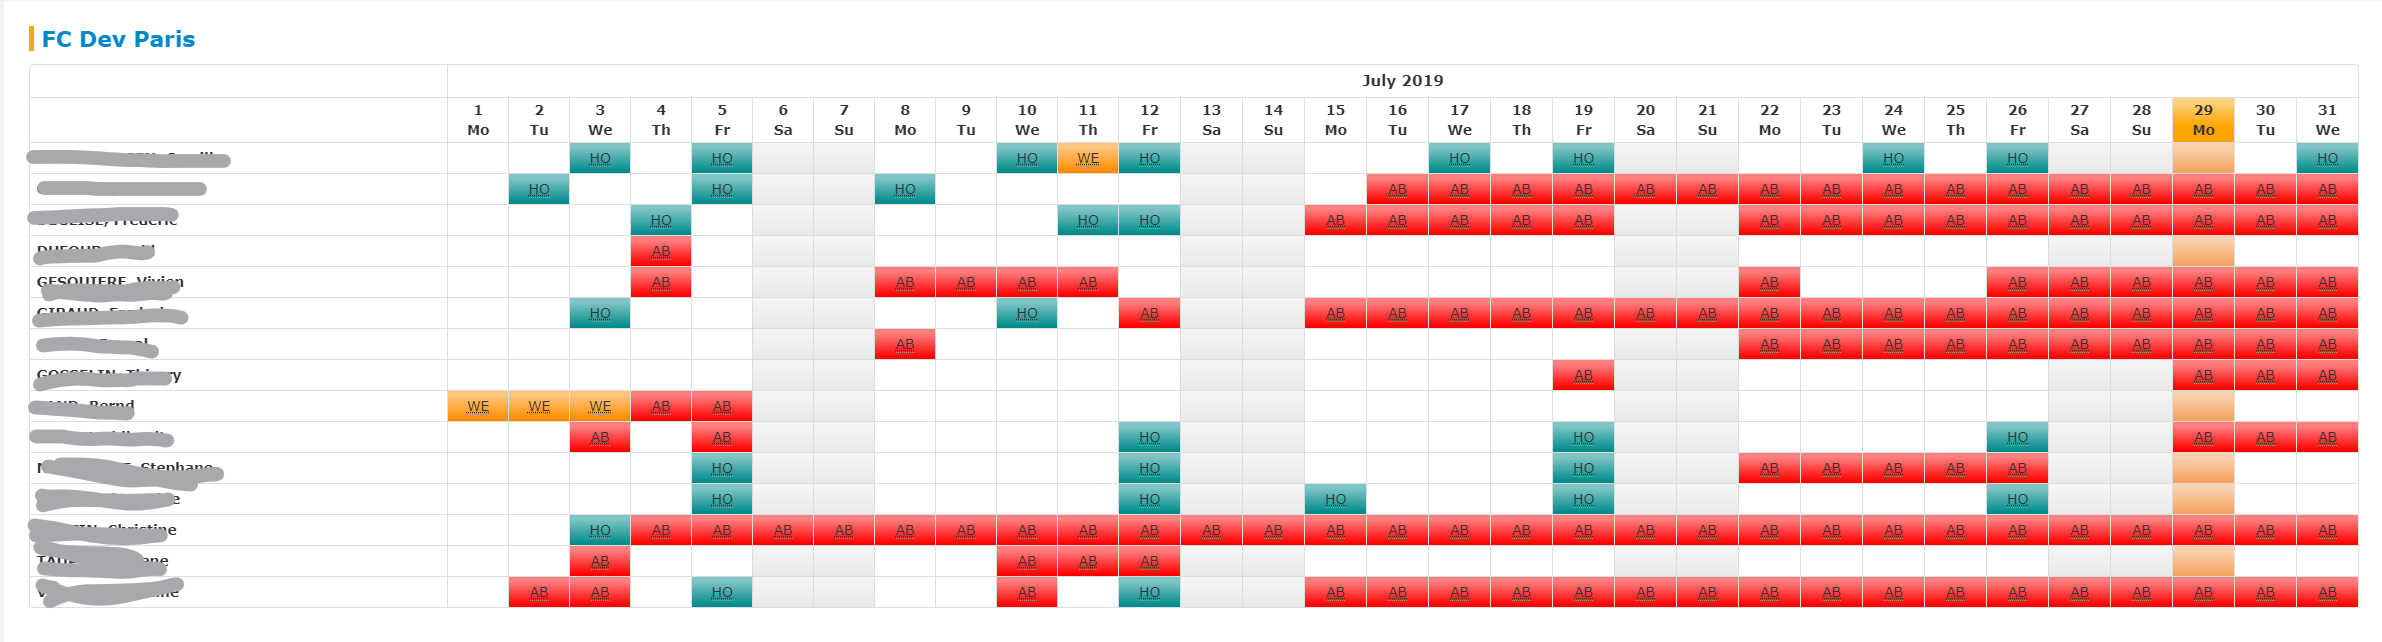
\includegraphics[width=\textwidth]{teamcalendar.png}
    	\caption{Caption}
    	\label{fig:teamCalendar_label}
    \end{figure}
    
%%%%%%%%%%%%%%%%%%%%%%%%%%%%%%%%%%%%%%%%%%%%%%%%%%%%%%%
\newpage
\section{Conclusion}
Après d'avoir suivi les cours théoriques à Sorbonne Université et à CFA INSTA, et d'avoir travaillé chez SAP France, je me sens beaucoup amélioré mes compétences sur le développement en Java, les connaissances sur les XPath, la compréhension théorique de Lambda Expression, des connaissances sur le domaine de finance.

\par Durant cette année d'alternance, j'ai appris beaucoup aussi sur la gestions de projet, sur la méthodologie de comment travailler ensemble dans une grande équipe, de comment travailler dans une petite sous-équipe, de comment être patient pour travailler, de comment travailler efficacement.

\par Pour finir, j'ai appris beaucoup de chose pendant cette année d'alternance et je me sens d'être à l'aise à SAP, c'est heureux d'effectuer mon alternance chez SAP. Et pendant ces années d'études en Master à Sorbonnes Université, j'ai appris aussi beaucoup de chose, pour ma vie, pour mon futur professionnel.


%%%%%%%%%%%%%%%%%%%%%%%%%%%%%%%%%%%%%%%%%%%%%%%%%
\newpage
\bibliography{biblist}
\newpage

%Rajouter la ligne "Annexes" dans le sommaire
\addcontentsline{toc}{part}{Annexes}

\begin{appendix}
\section{Annexe des codes}
    \subsection{Multi-Thread pour la comparaison des pdf}
    \label{appendix: multi-thread_compare_pdf}
    \begin{lstlisting}
    	// First Thread - Ref
		Thread_PDF_To_PNG thread_one = null;		
		try
		{
			thread_one = new Thread_PDF_To_PNG(1,bar,GeneralFuncs.normalizePath(ref_filePath));
			es.execute(thread_one);			
		}
		catch (Exception e)
		{
			throw new Exception("Cannot proceed with PDF extraction to PNG. " + e.getMessage());
		}
		es.isTerminated();
		// Second Thread - Res
		Thread_PDF_To_PNG thread_two=null;
		try
		{
			thread_two = new Thread_PDF_To_PNG(2,bar,GeneralFuncs.normalizePath(res_filePath));
			es.execute(thread_two);
			
		} catch (Exception e)	{
			throw new Exception("Cannot proceed with PDF extraction to PNG. " + e.getMessage());
		}
		try	{
			// Wait for the end of two thread
			System.out.println("Wait for the end of multi-thread pdf extraction");
			bar.await(); 
			bar = null;
		} catch (InterruptedException ex)		{ 
			throw new Exception("Error Message : " + ex.getMessage());
		}
    
    \end{lstlisting}
    
    \newpage
    \subsection{Lambda Expression pour comparaison entre deux répertoires}
    \label{appendix:lambda_compare_towFolder}
    \begin{lstlisting}
	public static void compareFolderRefAndSrc(String refFolder, String srcFolder) throws Exception
	{
		TestLogger.getInstance().beginCheckpoint("Ref folder: " + refFolder + " - Src foler: " + srcFolder);
		
		try
		{
			Path dirRef = Paths.get(refFolder);
			Path dirSrc = Paths.get(srcFolder);
			
			// filter the .pdf file
			List<Path> listRefPath = Files.list(dirRef)
					.filter(f -> f.toString().endsWith(".pdf"))
					.collect(Collectors.toList());
			
			for (int ii = 0; ii < listRefPath.size(); ii++)
			{
				Path refPath = listRefPath.get(ii);
				Path srcPath = Files.list(dirSrc).filter(path -> path.getFileName().equals(refPath.getFileName())).findFirst().get();
				comparePDF(refPath.toString(), srcPath.toString());
			}
		}
		catch (Exception e)
		{
			TestLogger.getInstance().logError(e.getMessage());
		}
		
		TestLogger.getInstance().endCheckpoint();
	}
    \end{lstlisting}
\end{appendix}\newpage

\end{document}